\chapter{Marco Teórico}\label{cap:marco_teorico}

Este capítulo establece los fundamentos formales sobre los que se asienta el resto del trabajo. El objetivo es triple: definir con precisión el problema que se aborda, dotarse de un modelo matemático adecuado para razonar sobre él y, con ese modelo, presentar los algoritmos que se compararán en el resto de la memoria.

La Sección~\ref{sec:definicion} define el problema ``desde fuera'', en términos de las \emph{entradas} que recibe un algoritmo de asignación y de las \emph{salidas} que se esperan de él, sin recurrir todavía a ningún formalismo. Se parte del problema clásico de asignación de tareas multi-robot (MRTA) y se enriquece con las particularidades del escenario abordado (coaliciones, ventanas de ejecución, heterogeneidad y restricciones de batería) hasta llegar a su versión bajo incertidumbre (MRTAU). La sección concluye introduciendo las dos dimensiones transversales que clasifican los enfoques de resolución: el momento del cómputo (\emph{online} frente a \emph{offline}) y la arquitectura de control (centralizada frente a descentralizada).

La Sección~\ref{sec:modelos} proporciona el modelado matemático. Se introduce, de forma incremental, la familia de los Procesos de Decisión de Markov: desde el modelo básico (MDP) hasta la variante semi-Markoviana generalizada, descentralizada y parcialmente observable que acabará capturando todas las características del problema. Cada modelo relaja o extiende una hipótesis del anterior, lo que motiva de forma natural la transición de uno al siguiente.

La Sección~\ref{sec:formalizacion} enlaza ambas piezas, formalizando el problema definido al principio como una instancia de los modelos anteriores. La correspondencia se construye también de manera incremental, añadiendo una hipótesis cada vez: la versión determinista se modela como un MDP, la versión bajo incertidumbre como un GSMDP y, finalmente, la versión distribuida ---núcleo de este trabajo--- como un DEC-POGSMDP.

Por último, la Sección~\ref{sec:algoritmos} presenta los algoritmos propuestos, que pueden leerse de forma unificada como distintas \emph{políticas de comunicación} que resuelven el mismo DEC-POGSMDP con grados crecientes de coordinación: desde los \textit{baselines} sin comunicación (Random y Greedy), pasando por los métodos de mercado basados en pujas (CBAA y CBBA), hasta la planificación distribuida que comunica distribuciones sobre los planes (Dec-MCTS).


% ===========================================================================
\section{Definición del problema} \label{sec:definicion} % ===========================================================================

Antes de elegir un formalismo con el que razonar sobre el problema conviene describirlo de forma autocontenida, en términos de las \emph{entradas} que recibe un algoritmo de asignación (la descripción de un escenario) y de las \emph{salidas} que se esperan de él (una solución válida y su calidad). En esta sección se presenta primero el problema de asignación de tareas multi-robot en su forma clásica (Sección~\ref{subsec:mrta}) y, sobre él, las particularidades que caracterizan el escenario abordado en este trabajo, incluyendo las fuentes de incertidumbre (Sección~\ref{subsec:mrtau}). Posteriormente se discuten dos dimensiones transversales que clasifican los enfoques de resolución: el momento del cómputo (Sección~\ref{subsec:online-offline}) y la arquitectura de control (Sección~\ref{subsec:centralizado-descentralizado}).


% --------------------------------------------------------------------------- 
\subsection{MRTA: el problema de asignación de tareas multi-robot} \label{subsec:mrta} % ---------------------------------------------------------------------------

El problema de asignación de tareas multi-robot (\textit{Multi-Robot Task Allocation}, MRTA) consiste, en su forma más elemental, en distribuir un conjunto de tareas $\mathcal{T}=\{T_1,\dots,T_m\}$ entre un conjunto de robots $\mathcal{R}=\{R_1,\dots,R_n\}$ de modo que se optimice una medida de rendimiento del equipo (ya sea el tiempo de ejecución, el número de tareas resueltas, la distancia recorrida o cualquier combinación de las mismas) ~\cite{gerkey2004taxonomy}. 

La taxonomía de Gerkey y Matarić~\cite{gerkey2004taxonomy} organiza las variantes de MRTA según tres ejes: el número de tareas que un robot puede ejecutar simultáneamente (\textit{single-task}, ST, frente a \textit{multi-task}, MT), el número de robots que requiere cada tarea (\textit{single-robot}, SR, frente a \textit{multi-robot}, MR) y el horizonte de la asignación (\textit{instantaneous assignment}, IA, frente a \textit{time-extended assignment}, TA). Trabajos posteriores ampliaron esta clasificación para capturar las dependencias entre tareas y agentes~\cite{korsah2013taxonomy} y las restricciones temporales y de orden~\cite{nunes2017taxonomy}.

El problema abordado en este trabajo se basa en el escenario propuesto por \red{CITA AL TUTOR??}. Es una versión enriquecida de MRTA con las siguientes particularidades:

\begin{itemize}
    \item \textbf{Robots \textit{sigle-task} (ST).} Los robots pueden ejecutar una única tarea en un determinado instante de tiempo.

    \item \textbf{Tareas \textit{multi-robot} (MT).} Cada tarea $T_j$ cuenta con un número requerido de robots para su ejecución (\textit{workers}) $q_j\in \{ 1, \dots, n\}$. Para completarse, $q_j$ robots compatibles deben coincidir en su ubicación durante un intervalo común. Esta característica introduce dependencias entre las planificaciones de distintos robots y sitúa el problema, en la taxonomía de Korsah et al.~\cite{korsah2013taxonomy}, en la clase de dependencias entre-planificaciones (\textit{cross-schedule dependencies}). 

   \item \textbf{Asignación con horizonte temporal (TA).} Los robots no reciben una única tarea, sino que planifican \emph{secuencias} de tareas a lo largo del tiempo. Los robots cuentan con acceso completo a la información del escenario incluyendo el conjunto completo de tareas a ejecutar y cómo estas tareas se irán ``abriendo'' y ``cerrando'' con el tiempo. De esta manera, cada robot puede planificar una ruta, aunque no se comprometa a ella, lo que convierte el problema en un problema de enrutamiento y planificación cercano al \textit{Vehicle Routing Problem} ~\cite{tothvigo2014vehicle}.   
   
   \item \textbf{Ventanas de ejecución.} Cada tarea $T_j$ solo puede ejecutarse dentro de un intervalo temporal $[t_j^s, t_j^l]$, donde $t_j^s$ represenra el instante más temprano en que puede iniciarse una tarea y $t_j^l$ es el instante límite para completar la tarea. La propiedad anterior junto a esta convierten el problema en uno aún más similar a \textit{Vehicle Routing Problem with Time Windows} (VRPTW) ~\cite{tothvigo2014vehicle}. 
   
    \item \textbf{Listas de compatibilidades (heterogeneidad).} Los robots son heterogéneos: cada robot $r_i$ posee un conjunto de compatibilidades, es decir, tareas que puede ejecutar. Esta tabla de compatibilidades se puede modelar como una función binaria $\textit{Cap} : \{(i,j) \in \mathbb{N} \times \mathbb{N} \mid 1 \leq i \leq n, 1 \leq j \leq m\} \to \{ 0, 1 \}$ donde $\textit{Cap}(i,j) = 1$ si el robot $R_i$ puede ejecutar la tarea $T_j$ y $\textit{Cap}(i,j) = 0$ en caso contrario.
    
    \item \textbf{Restricciones de batería y recarga.} Cada robot $R_i$ dispone de un nivel de batería $b_i$ (limitado por una capacidad máxima $B_i$) que se consume al desplazarse y al ejecutar tareas. Para evitar el agotamiento, los robots pueden acudir a un conjunto de estaciones de recarga $\mathcal{S}$, lo que añade decisiones logísticas adicionales al plan. El consumo de batería se puede modelar dentro de la función de utilidad de y las estaciones de recarga se pueden considerar como tareas con dependencias especiales.
\end{itemize}

Estas características permiten especificar formalmente una instancia del problema y el concepto de solución.

\begin{definicion}[Instancia de MRTA] \label{def:instancia} Una instancia del problema MRTA propuesto viene dada por la tupla $\langle\mathcal{R},\mathcal{T},\mathcal{S},\textit{Cap,}d\rangle$, donde:
\begin{itemize}
    \item $\mathcal{R}$ es el conjunto de robots, donde cada robot $R_i\in\mathcal{R}$ se describe por su ubicación inicial $x_i^0$, su capacidad de batería $B_i$, su velocidad de desplazamiento $v_i$ y su tasa de consumo de batería durante el desplazamiento $\textit{rate-}R_i$.

    \item $\mathcal{T}$ es el conjunto de tareas, donde cada tarea $t_j\in\mathcal{T}$ se describe por su ubicación $x_j$, su duración $d_j$, su ventana de ejecución $[t_j^s,t_j^l]$, su número de \textit{workers} requerido $q_j$, su recompensa $w_j$ y su tasa de consumo de batería durante la ejecución $\textit{rate-}T_j$.

    \item $\mathcal{S}$ es el conjunto de estaciones de recarga, donde cada estación $S_k \in \mathcal{S}$ viene dada por su ubicación $x_k$ y su tasa de recarga de batería $\textit{rate-}S_k$.

    \item $\textit{Cap}(\cdot,\cdot)$ es la función de compatibilidad.

    \item $d(\cdot,\cdot)$ es la función que asigna a cada par de ubicaciones la distancia entre ellas.
\end{itemize}    
\end{definicion}

\begin{definicion}[Solución y factibilidad] \label{def:solucion} Una solución es un \textbf{plan} $\pi$ que asigna a cada robot una secuencia ordenada de tareas y operaciones de recarga, junto con los instantes en que las emprende. La solución es \textbf{factible} si satisface simultáneamente: \begin{enumerate}   
    \item \emph{Compatibilidad}: todo robot asignado a una tarea es compatible con ella.   
    
    \item \emph{Coalición}: cada tarea ejecutada cuenta con exactamente $q_j$ robots compatibles presentes durante un intervalo de ejecución.
    
    \item \emph{Ventanas}: la ejecución de cada tarea respeta su intervalo $[t_j^s,t_j^l]$.   
    
    \item \emph{Energía}: el nivel de batería de cada robot se mantiene no negativo a lo largo de toda su ruta, considerando consumos y recargas. 
    
    \item \emph{Secuenciación}: cada robot ejecuta una sola tarea a la vez, de forma coherente con los tiempos de desplazamiento. 
\end{enumerate} 
\end{definicion}

La calidad de una solución factible se evalúa mediante una \textbf{función de utilidad} de naturaleza cooperativa y multiobjetivo, que premia el número de tareas completadas y el número de robots que preservan su integridad (no agotan la batería), y penaliza el tiempo total de ejecución (\textit{makespan}) y el número de tareas que quedan pendientes. Una formulación habitual es 
\begin{equation} \label{eq:objetivo} 
U(\pi) \;=\; \lambda_c \sum_{T_j\in\mathcal{T}_{\mathrm{comp}}} w_j \;-\; \lambda_p\, |\mathcal{T}_{\mathrm{pend}}|   \;+\; \lambda_s\, n_{\mathrm{surv}}     \;-\; \lambda_t\, C_{\max}, 
\end{equation} 
donde $\mathcal{T}_{\mathrm{comp}}$ y $\mathcal{T}_{\mathrm{pend}}$ son los conjuntos de tareas completadas y pendientes, $n_{\mathrm{surv}}$ es el número de robots que finalizan sin agotar su batería, $C_{\max}$ es el \textit{makespan} y $\lambda_c,\lambda_s,\lambda_t,\lambda_p\ge 0$ ponderan los distintos objetivos, con $\lambda_c+\lambda_s+\lambda_t+\lambda_p = 1$. El objetivo del algoritmo es, por tanto, hallar el plan $\pi^*$ que maximice $U$.


% --------------------------------------------------------------------------- 
\subsection{MRTAU: el problema bajo incertidumbre} \label{subsec:mrtau} % ---------------------------------------------------------------------------

La formulación anterior es \emph{determinista}: supone que los tiempos de desplazamiento, las duraciones de las tareas, el consumo de energía y el éxito de cada ejecución son conocidos de antemano y se cumplen con exactitud. En un sistema robótico real esta hipótesis no se sostiene. La variante \emph{MRTAU} (MRTA \textit{under Uncertainty}) añade a la Definición~\ref{def:instancia} las siguientes fuentes de incertidumbre:

\begin{enumerate}  
    \item \textbf{Resultado de tareas incierto.} La ejecución de una tarea puede fracasar: tras comenzar la ejecución de una tarea $T_j$, ésta se completa con éxito con cierta probabilidad $\rho_j$ y fracasa con probabilidad $1-\rho_j$. 
    
    \item \textbf{Duraciones de tarea estocásticas.} La duración de ejecutar una tarea es igualmente aleatoria. Las tareas cuentan con una distribución de probabilidad de tiempo de ejecución $\mathcal{N}(\mu_t^s, \sigma_t^s)$ en caso de éxito y una distinta $\mathcal{N}(\mu_t^f, \sigma_t^f)$ en caso de fracaso.
      
    \item \textbf{Consumo de batería estocástico.} Debido a la estocasticidad de los tiempos de ejecución de las tareas, el consumo de batería durante la ejecución también está sujeto a variabilidad, lo que vuelve incierta la viabilidad energética de cualquier tarea. \end{enumerate}

La consecuencia de introducir estas fuentes de incertidumbre es profunda y condiciona todo el trabajo: una solución entendida como un plan fijo calculado de antemano deja de ser adecuada. Un plan que parezca factible respecto a los valores nominales puede violar una ventana de ejecución porque un desplazamiento tardó más de lo previsto, o dejar a un robot sin batería por un consumo mayor del esperado. En consecuencia, el concepto de solución se desplaza de un \emph{plan estático} a una \emph{política adaptativa}: una regla que decide la siguiente acción de cada robot en función de los resultados estocásticos que se van observando. Esta observación motiva tanto el empleo de algoritmos que computan durante la ejecución (Sección~\ref{subsec:online-offline}) como la formalización del problema mediante procesos de decisión secuencial bajo incertidumbre, que se aborda en las Secciones~\ref{sec:modelos} y~\ref{sec:formalizacion}.

En este nuevo paradigma, es indispensable establecer una diferencia entre una política y un episodio, y consecuentemente, entre la función de utilidad y la función de recompensa:
\begin{itemize}
    \item \textbf{Episodio ($\xi$):} Representa una realización concreta del sistema \textit{multi-robot} desde el estado inicial hasta un posible estado final. Debido a la naturaleza estocástica del entorno, la ejecución secuencial de una misma política dará lugar a múltiples episodios posibles, cada uno con diferentes duraciones de tareas o fallos imprevistos. Cada episodio individual se evalúa mediante una \textbf{función de recompensa} del episodio $R(\xi)$:
    \begin{equation} \label{eq:recompensa}
    R(\xi) \;=\; \lambda_c \sum_{T_j\in\mathcal{T}_{\mathrm{comp}}} w_j \;-\; \lambda_p\, |\mathcal{T}_{\mathrm{pend}}|   \;+\; \lambda_s\, n_{\mathrm{surv}}     \;-\; \lambda_t\, C_{\max}, 
    \end{equation}
    Al depender de la incertidumbre, $R(\xi)$ se comporta como una variable aleatoria.
    
    \item \textbf{Política ($\pi$):} Representa la estrategia o reglas de decisión que rigen las decisiones de los robots. Una política no puede evaluarse justamente a través de un único episodio aislado debido a la variabilidad del entorno. En su lugar, se evalúa mediante la \textbf{función de utilidad} $U(\pi)$, la cual se define como la esperanza matemática de las recompensas de todos los episodios que dicha política es capaz de generar:
    \begin{equation} \label{eq:utilidad_esperada}
    U(\pi) \;=\; \mathbb{E}_{\xi \sim \pi} \left[ R(\xi) \right]
    \end{equation}
    donde la esperanza se calcula sobre la distribución de probabilidad de las trayectorias $\xi$ inducidas por la política $\pi$. El objetivo en el problema MRTAU se convierte, por tanto, en hallar la política óptima $\pi^*$ que maximice la utilidad esperada $U(\pi)$.
\end{itemize}


% --------------------------------------------------------------------------- 
\subsection{Algoritmos \textit{online} frente a \textit{offline}} \label{subsec:online-offline} % ---------------------------------------------------------------------------

Definido el problema, conviene introducir dos criterios que clasifican los enfoques de resolución. El primero concierne a \emph{cuándo} se calcula la solución en relación con su ejecución. Un algoritmo \textbf{\textit{offline}} (o de planificación \textit{a priori}) construye la solución completa antes de que comience la ejecución, asumiendo un modelo completo y estático del problema. Una vez calculada, la solución se ejecuta sin modificaciones. Este paradigma es adecuado cuando el entorno es determinista y conocido, y cuando el coste de la planificación puede asumirse fuera del bucle de ejecución. Su limitación fundamental es la fragilidad ante la incertidumbre: cualquier desviación entre el modelo empleado para planificar y la realidad observada arruina la solución calculada a priori.

Un algoritmo \textbf{\textit{online}} (o reactivo), por el contrario, intercala el cómputo con la ejecución: las decisiones se toman de manera adaptativa a medida que se dispone de nueva información. Esto permite reaccionar ante los eventos estocásticos descritos en la Sección~\ref{subsec:mrtau} (el fallo de una tarea, un retraso o un consumo imprevisto) replanificando con el estado más reciente. La contrapartida es que el tiempo de cómputo en cada decisión está acotado, por lo que estos métodos se apoyan en heurísticas o en algoritmos de tipo \textit{anytime} debidamente optimizados, capaces de devolver una solución factible en cualquier instante y de mejorarla si se les concede más tiempo. El algoritmo de búsqueda \textit{Monte Carlo Tree Search} (MCTS) es el ejemplo perfecto de método \textit{online} \textit{anytime}~\cite{browne2012survey}.

Dado que el problema MRTAU combina incertidumbre y tiempos continuos, un enfoque puramente \textit{offline} resulta inviable: el espacio de contingencias posibles crece de forma combinatoria y no puede enumerarse por anticipado. Por ello, los algoritmos considerados en este trabajo son esencialmente \textit{online}, en línea con el modelo base de \red{CITA AL TUTOR}.


% --------------------------------------------------------------------------- 
\subsection{Algoritmos centralizados frente a descentralizados} \label{subsec:centralizado-descentralizado} % ---------------------------------------------------------------------------

El segundo criterio de clasificación concierne a \emph{quién} toma las decisiones y de \emph{qué} información dispone para hacerlo. En una arquitectura \textbf{centralizada} existe una entidad coordinadora (un planificador único) con acceso al estado de todos los robots y todas las tareas, que calcula la asignación para el conjunto de robots completo y comunica a cada robot las acciones que debe ejecutar. Su ventaja teórica es la posibilidad de alcanzar la solución óptima global, al razonar sobre información completa. Sus inconvenientes son conocidos: constituye un único punto de fallo, escala de forma deficiente con el número de agentes (el espacio de decisiones conjunto crece exponencialmente) y exige comunicación fiable y de baja latencia con todos los robots.

En una arquitectura \textbf{descentralizada} (o distribuida) no existe tal entidad: cada robot es un agente autónomo que decide sus acciones a partir de su información \emph{local} (su propio estado y, eventualmente, los mensajes que recibe de sus vecinos), sin acceso directo al estado interno de los demás. La coordinación, cuando es necesaria, emerge del intercambio explícito de información. Esta arquitectura es intrínsecamente robusta, escala mejor y se adapta a escenarios con comunicación limitada o intermitente. Su precio es la pérdida de la garantía de optimalidad global: al razonar sobre información parcial, los agentes pueden tomar decisiones localmente racionales pero globalmente subóptimas, y pueden surgir conflictos (por ejemplo, dos robots que se dirigen a la misma tarea) que deben resolverse mediante mecanismos de consenso~\cite{dias2006market}. 

\begin{table}[t] \centering \caption{Compromisos entre arquitecturas de control para MRTA.} \label{tab:cent-vs-desc} \begin{tabular}{lcc} \hline \textbf{Criterio} & \textbf{Centralizado} & \textbf{Descentralizado} \\ \hline Información disponible      & Estado global & Estado local + mensajes \\ Optimalidad         & Óptimo global posible & Subóptimo (en general) \\ Robustez ante fallos        & Punto único de fallo  & Tolerante a fallos \\ Escalabilidad       & Pobre         & Buena \\ Coste de comunicación       & Alto y centralizado   & Distribuido y acotado \\ \hline \end{tabular} \end{table}

La Tabla~\ref{tab:cent-vs-desc} resume estos compromisos. El presente trabajo adopta deliberadamente el paradigma descentralizado: partiendo del modelo centralizado de \red{CITA AL TUTOR}, el objetivo es transitar hacia una resolución puramente distribuida. Como se justifica en la Sección~\ref{sec:formalizacion}, esta transición no es un mero detalle de implementación: la ausencia de observabilidad global cambia la naturaleza formal del problema y obliga a sustituir la información compartida por mecanismos de coordinación basados en comunicación.


% =========================================================================== 
\section{Procesos de Decisión de Markov} \label{sec:modelos} % ===========================================================================

La toma de decisiones secuencial bajo incertidumbre se modela habitualmente mediante la familia de los Procesos de Decisión de Markov (\textit{Markov Decision Process}). En esta sección se introducen, de forma incremental, los cinco modelos relevantes para este trabajo. Cada uno relaja o extiende una hipótesis del anterior: partiendo de un modelo inicial MDP (Sección~\ref{subsec:mdp}), el POMDP elimina la observabilidad total (Sección~\ref{subsec:pomdp}), el SMDP elimina el tiempo discreto (Sección~\ref{subsec:smdp}). En este punto se planteará el problema fundamental que surge al aplicar el SMDP a un escenario con acciones concurrentes y continuas (el \emph{leak temporal}), el GSMDP surge como una respuesta al problema (Sección~\ref{subsec:gsmdp}). Por último, el DEC-POSMDP combina todas estas características dentro de un contexto multi-agente descentralizado (Sección~\ref{subsec:decposmdp}). Esta progresión guiará la formalización de la Sección~\ref{sec:formalizacion}.


% --------------------------------------------------------------------------- 
\subsection{Proceso de Decisión de Markov (MDP)} \label{subsec:mdp} % ---------------------------------------------------------------------------

El \emph{Proceso de Decisión de Markov} es el modelo fundamental para la toma de decisiones secuencial en entornos estocásticos pero completamente observables~\cite{bellman1957dynamic,puterman1994markov}.

\begin{definicion}[MDP] \label{def:mdp} 
Un Proceso de Decisión de Markov es una tupla $\langle\mathcal{S},\mathcal{A},\mathcal{T},\mathcal{R},\gamma\rangle$ donde: 
\begin{itemize}   
    \item $\mathcal{S}$ es un conjunto finito de \textbf{estados}.   
    
    \item $\mathcal{A}$ es un conjunto finito de \textbf{acciones}.   
    \item $\mathcal{T}:\mathcal{S}\times\mathcal{A}\times\mathcal{S}\to[0,1]$ es la \textbf{función de transición}, donde $\mathcal{T}(s,a,s')=P(s_{k+1}=s'\mid s_k=s,a_k=a)$ define la probabilidad de alcanzar el estado $s'$ al aplicar la acción $a$ desde el estado $s$.
    
    \item $\mathcal{R}:\mathcal{S}\times\mathcal{A}\to\mathbb{R}$ es la \textbf{función de recompensa} que atribuye un valor real $\mathcal{R}(s,a)$ a cada acción $a$ tomada en un determinado estado $s$, ayudando al agente a priorizar aquellas acciones que maximicen su beneficio a largo plazo.
    
    \item $\gamma\in[0,1]$ es el \textbf{factor de descuento}, que pondera la importancia de las recompensas futuras frente a las inmediatas. Un valor $\gamma \to 0$ indica a los agentes a priorizar recompensas inmediatas mientras que un valor $\gamma \to 1$ favorece las recompensas futuras.
\end{itemize} 
\end{definicion}

La hipótesis central que da nombre al modelo es la \textbf{propiedad de Markov}: la distribución del estado siguiente depende únicamente del estado y la acción actuales, y no de la historia previa, \begin{equation} 
P(s_{k+1}\mid s_k,a_k,\dots,s_0,a_0)=P(s_{k+1}\mid s_k,a_k). 
\end{equation} 

En este contexto, una solución a este problema es una \textbf{política}, esto es, una función $\pi : \mathcal{S} \to \mathcal{A}$ que, dado un estado, devuelva una acción a aplicar.

El objetivo es hallar una política que maximice la recompensa acumulada esperada. La calidad de una política se mide mediante la \textbf{función de utilidad} $U_\pi$, que satisface la ecuación de Bellman~\cite{bellman1957dynamic}: 
\begin{equation} \label{eq:bellman} 
U_\pi(s)=\mathcal{R}(s,\pi(s)) +\gamma\sum_{s'\in\mathcal{S}}\mathcal{T}(s,\pi(s),s')\,U_\pi(s'). 
\end{equation}

La política óptima $\pi^\ast$ es la que maximiza $U_\pi(s)$ en todo estado. Dos hipótesis implícitas del MDP serán relajadas más adelante: (i) el agente observa el estado completo en cada instante y (ii) las transiciones ocurren en pasos de tiempo discretos y unitarios. Es por eso que es necesario introducir los siguientes modelos.


% --------------------------------------------------------------------------- 
\subsection{Proceso de Decisión de Markov Parcialmente Observable (POMDP)} \label{subsec:pomdp} % ---------------------------------------------------------------------------

En numerosos problemas el agente no conoce directamente el estado del sistema, sino observaciones parciales y posiblemente ruidosas a partir de las cuales debe inferirlo. El \textbf{POMDP} (\textit{Partially Observable Markov Decision Process}) extiende el MDP para capturar esta limitación~\cite{kaelbling1998planning}.

\begin{definicion}[POMDP] \label{def:pomdp} 
Un Proceso de Decisión de Markov Parcialmente Observable es una tupla $\langle\mathcal{S},\mathcal{A},\mathcal{T},\mathcal{R},\Omega,\mathcal{O}, \gamma\rangle$ donde: 
\begin{itemize}   
    \item $\mathcal{S}$, $\mathcal{A}$, $\mathcal{T}$, $\mathcal{R}$ y $\gamma$ describen un MDP (Definición~\ref{def:mdp}).
    \item $\Omega$, un conjunto finito de todas las posibles \textbf{observaciones}.   
    \item $\mathcal{O}:\mathcal{S}\times\mathcal{A}\times\Omega\to[0,1]$, la \textbf{función de observación}, donde $\mathcal{O}(s',a,o)=P(o_{k+1}=o\mid s_{k+1}=s',a_k=a)$ es la probabilidad de percibir la observación $o$ una vez se alcanza el estado $s'$ tras aplicar la acción $a$. 
\end{itemize} 
\end{definicion}

El agente no conoce el estado actual del entorno, por lo que mantiene una \textbf{creencia} (\textit{belief}) $b\in\Delta(\mathcal{S})$: una distribución de probabilidad sobre los estados posibles. La creencia es un estadístico suficiente de toda la historia de acciones y observaciones, y se actualiza de forma bayesiana tras cada par $(a,o)$: \begin{equation} \label{eq:belief-update} 
b'(s')=\eta\,\mathcal{O}(s',a,o)\sum_{s\in\mathcal{S}}\mathcal{T}(s,a,s')\,b(s), 
\end{equation} 
donde $\eta$ es un factor de normalización que garantiza que la suma de probabilidades sea $1$. Esta
actualización combina la creencia a priori de un agente sobre el entorno dinámico $\mathcal{T}(s,a,s')\,b(s)$ con la nueva observación obtenida $\mathcal{O}(s',a,o)$, permitiendo al agente refinar progresivamente su conocimiento sobre el estado real. 
Un agente se puede descomponer en dos partes, como muestra la Figura~\ref{fig:pomdp}.
\begin{figure}
    \centering
    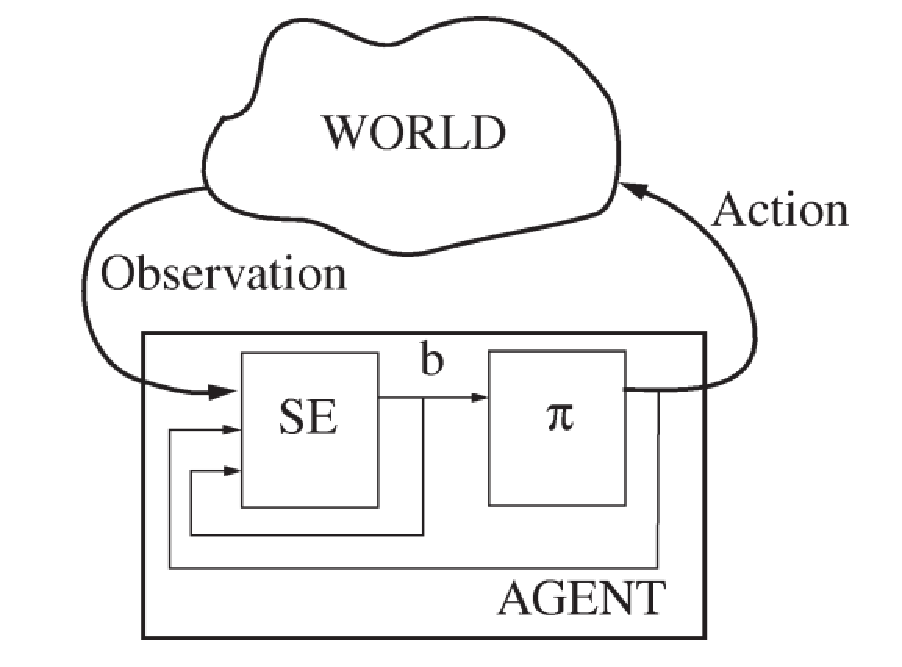
\includegraphics[width=0.5\linewidth]{figures/02_marco_teórico/pomdp.pdf}
    \caption{En un POMDP, un agente se puede descomponer en un \textit{estimador de estado} (SE) y una \textit{política} ($\pi$).}
    \label{fig:pomdp}
\end{figure}

El objetivo de un agente en un POMDP, al igual que en un MDP, es encontrar una política óptima $\pi^\ast$ que maximice recompensa acumulada esperada. Sin embargo, en este caso, la política se define sobre los estados de creencia y no sobre los estados físicos del sistema, ya que el agente no puede observarlos directamente. Un POMDP puede reformularse como un MDP sobre el espacio de creencias (\emph{belief-MDP}); el inconveniente es que dicho espacio es continuo y de dimensión $|\mathcal{S}|-1$, lo que hace que la resolución exacta sea intratable en el caso general~\cite{kaelbling1998planning}. Es por eso que, para abordar esta dificultad, se han propuesto numerosas estrategias de aproximación.


% --------------------------------------------------------------------------- 
\subsection{Proceso de Decisión Semi-Markoviano (SMDP)} \label{subsec:smdp} % ---------------------------------------------------------------------------

Los modelos anteriores asumen que el tiempo avanza en pasos discretos y que toda acción consume una unidad temporal. Esto es inadecuado cuando las acciones tienen duraciones variables y continuas, como desplazarse, ejecutar una tarea o recargar. El SMDP (\textit{Semi-Markov Decision Process}) generaliza el MDP permitiendo que el tiempo de permanencia en cada estado (o el tiempo de transición entre estados; son dos maneras de interpretar una misma formalidad) sea una variable aleatoria de valor real~\cite{howard1971dynamic}.

\begin{definicion}[SMDP] \label{def:smdp} Un Proceso de Decisión Semi-Markoviano es una tupla $\langle\mathcal{S},\mathcal{A},\mathcal{F},\mathcal{R},\gamma\rangle$ que generaliza la Definición~\ref{def:mdp} mediante una \textbf{distribución conjunta de transición y duración} 
\begin{equation} 
\mathcal{F}(s',\tau\mid s,a)=P(s_{k+1}=s',\,\tau_k\le\tau\mid s_k=s,a_k=a), \end{equation} 
que describe simultáneamente la probabilidad de transitar a $s'$ y la distribución del tiempo continuo $\tau\in [0, +\infty)$ que tarda en producirse la transición. La función de transición discreta del MDP se recupera como la marginal $\mathcal{T}(s,a,s')=\lim_{\tau\to\infty}\mathcal{F}(s',\tau\mid s,a)$. Adicionalmente, se sustituye el factor de descuento discreto $\gamma \in (0,1)$ por una \textbf{tasa de descuento continua} $\beta > 0$, que permite aplicar un descuento en función del tiempo de transición.
\end{definicion}

La denominación \emph{Semi-Markoviano} surge de una relajación de la propiedad de Markov. En un MDP clásico, el futuro del sistema depende exclusivamente del estado actual. En un SMDP, dado que las acciones tienen una duración continua $\tau$, el tiempo que el agente lleva ejecutando una acción puede afectar al estado resultante de la misma.

Por ejemplo, si un robot inicia la acción de trasladarse a un pasillo lejano (cuya duración típica es de 10 segundos) y se analiza el sistema transcurridos 9 segundos, la probabilidad de alcanzar el estado destino de forma inminente es mayor que si acabara de comenzar la acción. En consecuencia, la propiedad de Markov se viola durante el transcurso de la acción. Sin embargo, la propiedad de Markov se recupera por completo en los instantes de decisión (es decir, en los momentos clave en los que una acción concluye, se alcanza un nuevo estado $s'$ y el agente debe elegir la siguiente acción $a$).

Esta naturaleza continua altera la formulación de la \textbf{función de utilidad}. En el caso discreto, la ecuación de Bellman representa conceptualmente una esperanza matemática ($\mathbb{E}_{s'}$) sobre el conjunto discreto de estados futuros del sistema. La Ecuación~\ref{eq:bellman} es equivalente a:
\begin{equation} \label{eq:bellman2}
    U_\pi(s) = \mathbb{E}_{s'}\!\left[\, \mathcal{R}(s,\pi(s)) + \gamma \, U_\pi(s') \mid s, \pi(s) \,\right]
\end{equation}

Al transicionar al paradigma SMDP, el estado futuro ya no depende de un único paso temporal, sino de dos variables aleatorias conjuntas: el estado de destino $s'$ (discreto) y el tiempo de transición $\tau$ (continuo). De este modo, la ecuación de Bellman para un SMDP bajo un horizonte descontado se establece como:
\begin{equation} \label{eq:bellman-smdp} 
U_\pi(s)=\mathbb{E}_{s',\tau}\!\left[\,\mathcal{R}(s,\pi(s)) +e^{-\beta\tau}\,U_\pi(s')\,\middle|\,s,\pi(s)\right].
\end{equation}
En esta fórmula, el factor de descuento se modela mediante una función exponencial negativa $e^{-\beta\tau}$. 

No obstante, el SMDP asume implícitamente que en cada instante hay una única acción activa, cuya finalización constituye el siguiente instante de decisión. En un sistema \textit{multi-robot} esta hipótesis se rompe (las acciones de distintos robots se solapan en el tiempo), y al intentar aplicar el SMDP en esas condiciones surge un problema que conviene plantear con precisión, pues condiciona todos los modelos posteriores.


% --------------------------------------------------------------------------- 
\subsection{Proceso de Decisión Semi-Markoviano Generalizado (GSMDP)} \label{subsec:gsmdp} % ---------------------------------------------------------------------------
 
\paragraph{La fuga de información temporal (\emph{leak temporal}).} Considérese la situación de la Figura~\ref{fig:leak}: el robot $R_1$ está ejecutando la tarea $T_1$, iniciada en un instante anterior, y en el instante de decisión $t_k$ el robot $R_2$ queda libre y debe elegir su siguiente acción. La maquinaria del SMDP asocia a cada acción el núcleo $\mathcal{F}(s',\tau\mid s,a)$, que en el momento en que la acción comienza determina conjuntamente el estado de destino $s'$ y la duración $\tau$. Si esa duración (o, de forma equivalente, el instante de finalización ya muestreado) se almacena en el estado, entonces en $t_k$ el estado contiene el instante exacto en que $T_1$ concluirá y $R_1$ se liberará. La política de $R_2$, que decide en función del estado global, accedería así a información sobre un evento futuro que en una ejecución real todavía no se ha producido. Esta fuga de información, que denominaremos \emph{leak temporal}, es una limitación intrínseca del SMDP en presencia de concurrencia y observabilidad total. La única salida es desacoplar la información que el modelo necesita internamente de la que la política puede observar: un mecanismo de
eventos con relojes ocultos. Ese mecanismo es el del GSMP.
 
\begin{figure}
    \centering
    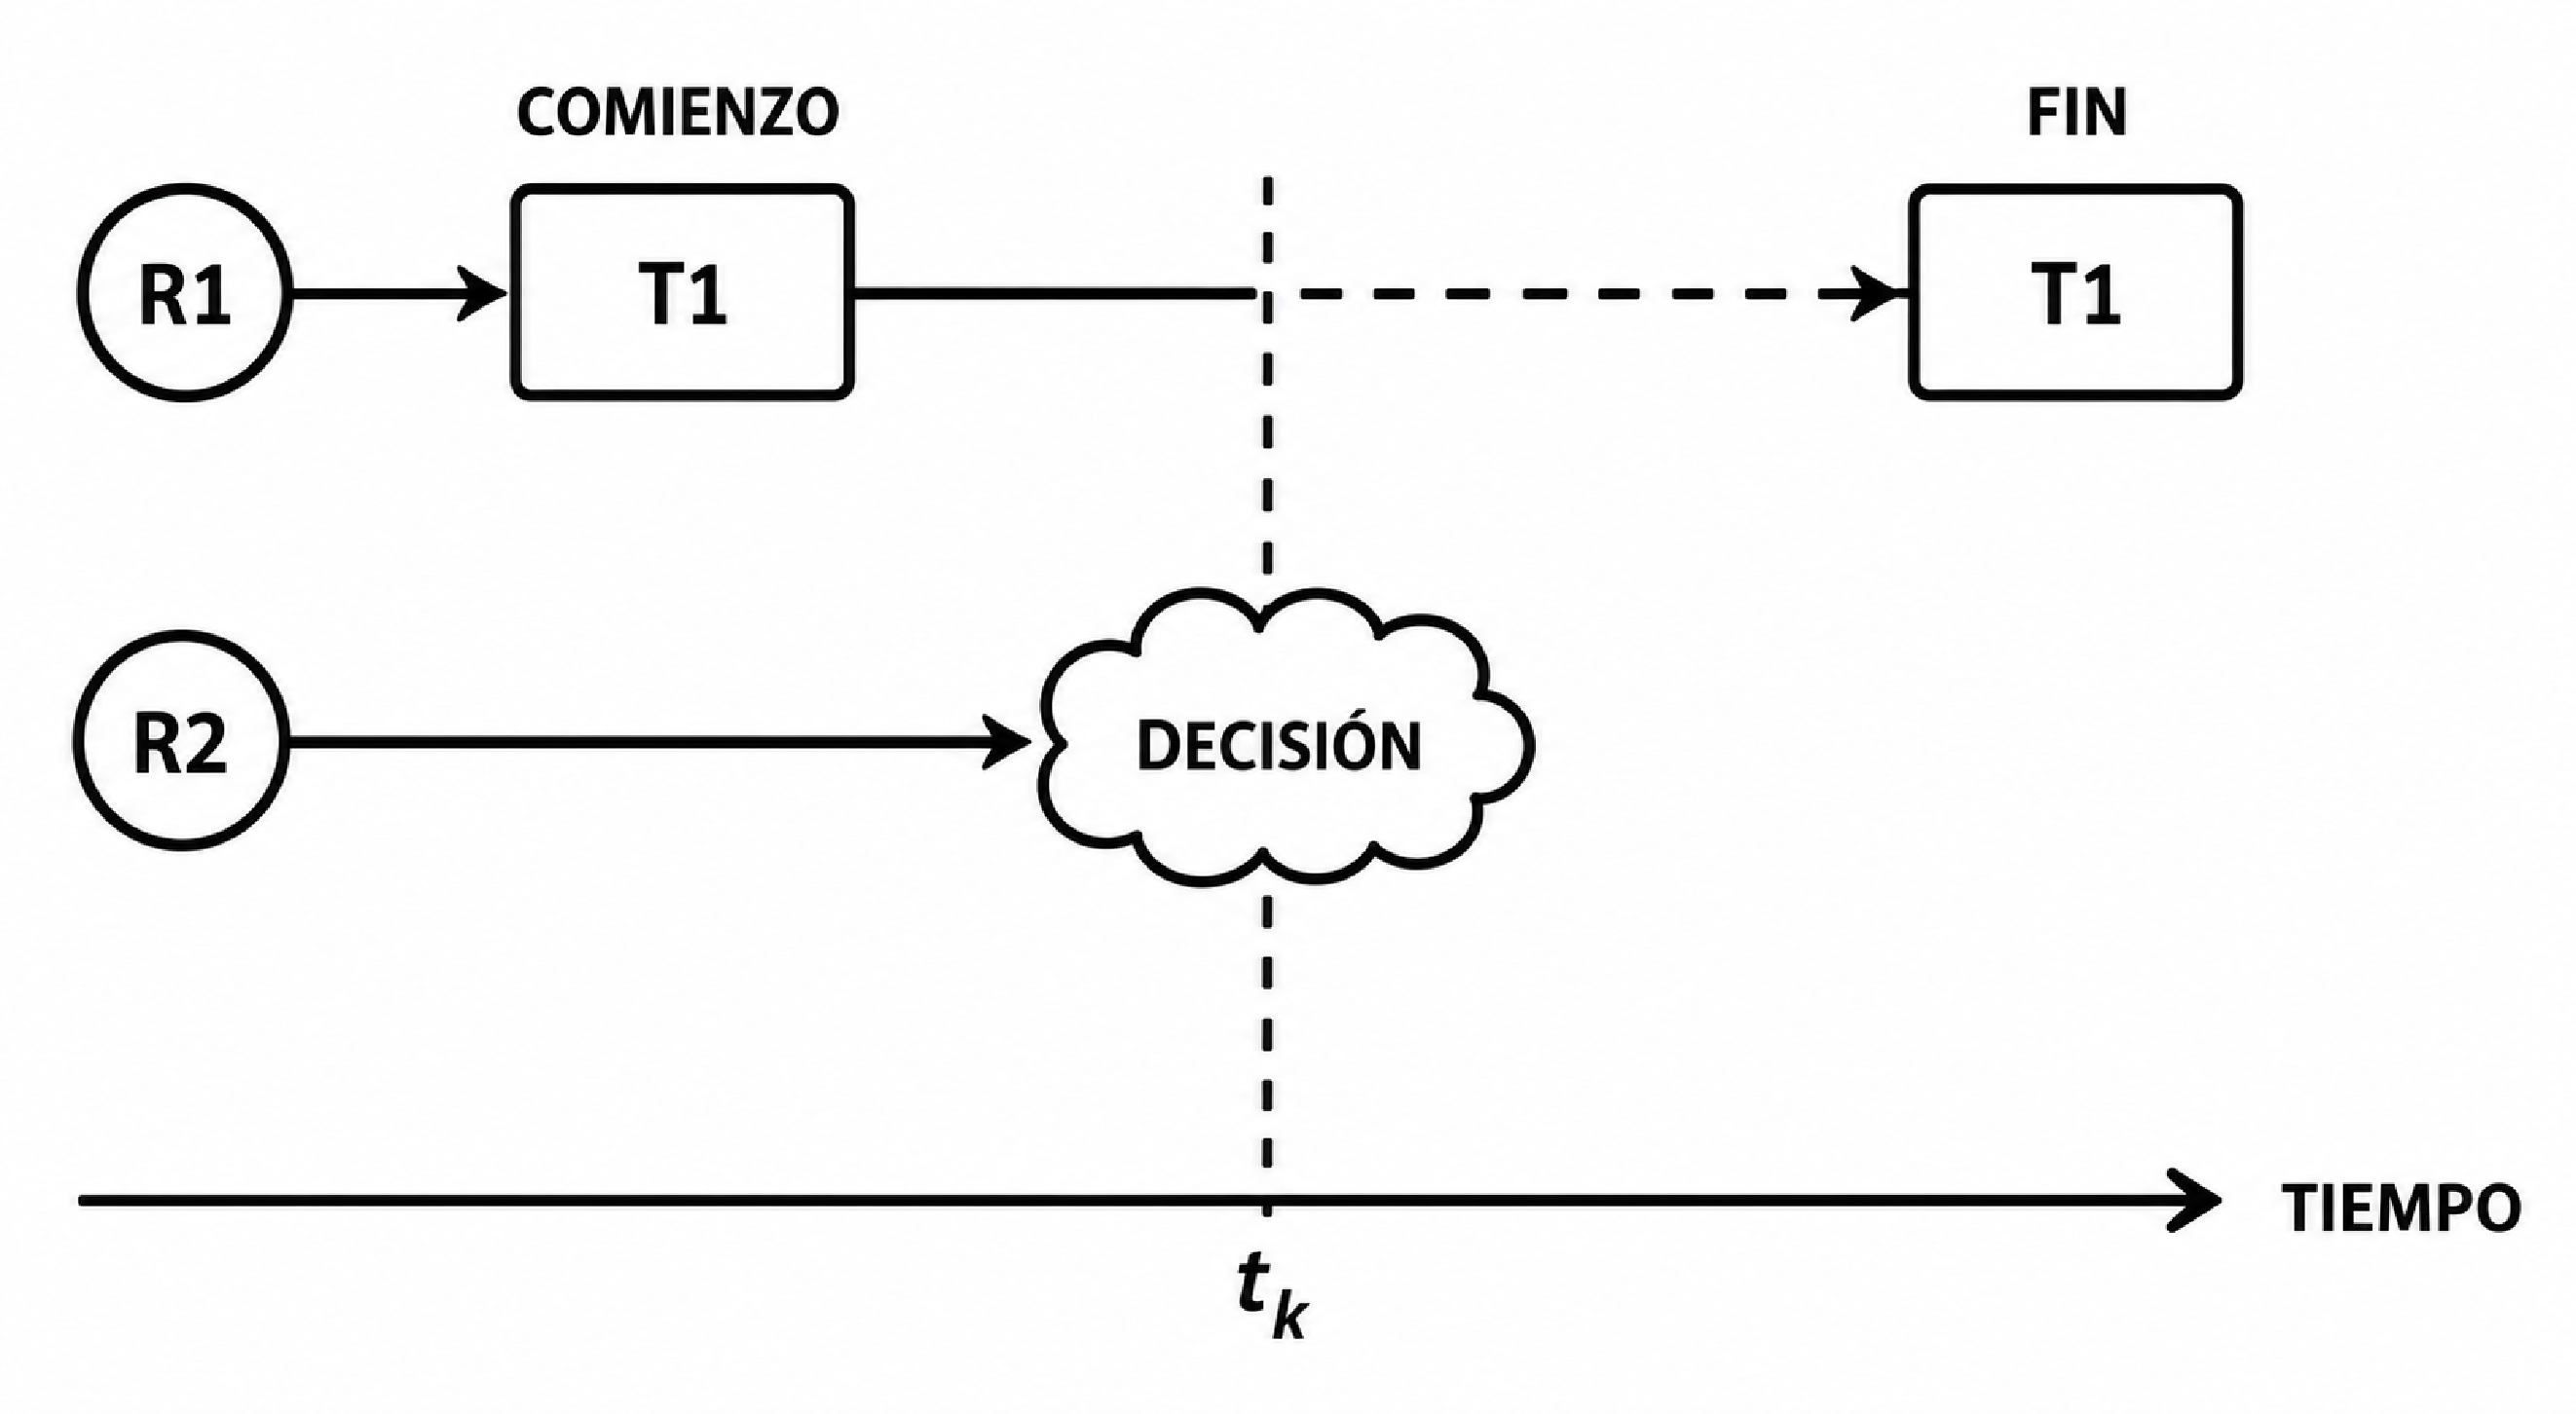
\includegraphics[width=0.85\linewidth]{figures/02_marco_teórico/data_leakage.pdf}
    \caption{Ilustración del \emph{leak temporal}. En el instante $t_k$, el robot $R_2$ debe decidir su siguiente acción mientras $R_1$ ejecuta la tarea $T_1$, comenzada con anterioridad. Sin embargo, el instante de finalización de $T_1$ (el evento \textsc{FIN}, aún no producido) ya se ha muestreado y guardado en el estado al \textsc{COMIENZO} de la tarea, la decisión de $R_2$ podría depender de información futura que no estaría disponible en una ejecución real.}
    \label{fig:leak}
\end{figure}
 
El \emph{Proceso de Decisión Semi-Markoviano Generalizado} (GSMDP)~\cite{younes2004gsmdp}, construido sobre el formalismo del \emph{Proceso Semi-Markoviano Generalizado} (GSMP)~\cite{glynn1989gsmp}, resuelve el problema ambos al modelar el solapamiento de acciones mediante eventos con relojes, ocultos para el agente.
 
\begin{definicion}[GSMP y GSMDP] \label{def:gsmdp}
Un \emph{Proceso Semi-Markoviano Generalizado} (GSMP) modela el sistema mediante un conjunto de \textbf{eventos}. En cada estado discreto $s$ hay un subconjunto $\mathcal{E}(s)$ de eventos \emph{activos}. A cada evento activo $e \in \mathcal{E}(s)$ se le asocia un \textbf{reloj} cuyo tiempo de disparo $\tau_e$ se muestrea de su distribución $F_e$ en el momento en que el evento se activa. Los relojes avanzan en paralelo y el evento cuyo reloj expira primero,
\begin{equation}
    e^* = \arg\min_{e\,\in\,\mathcal{E}(s)}\,\tau_e,
\end{equation}
desencadena la transición al siguiente estado $s'$. Los relojes de los eventos que permanecen activos en $s'$ conservan su tiempo transcurrido  y los de los eventos recién activados en $s'$ se muestrean de nuevo. El \emph{Proceso de Decisión Semi-Markoviano Generalizado} (GSMDP) extiende el GSMP añadiendo que algunos eventos son \textbf{controlables} por el decisor (las acciones $a \in \mathcal{A}$).
\end{definicion}
 
La representación por relojes resuelve el dilema anterior y ofrece, por tanto, una doble ventaja. En primer lugar, el valor muestreado de cada reloj $\tau_e$ es una variable \emph{latente} del modelo: la política condiciona únicamente sobre el estado discreto y sobre los tiempos transcurridos $\delta_e$, nunca sobre los instantes de disparo todavía no realizados. Esto elimina el \emph{leak temporal}. En segundo lugar, al modelar el tiempo de finalización de las acciones en el conjunto de eventos, ahora el estado global puede almacenar los tiempos transcurridos de las acciones $\delta_e$. Las duraciones de las acciones no son, en general, sin memoria (en este trabajo se modelan como gaussianas). En consecuencia, el tiempo restante de una acción en curso depende del tiempo que ya lleva ejecutándose: como ilustra la Figura~\ref{fig:cond-prob}, la esperanza de la duración total $\mathbb{E}[X]$ difiere de la esperanza condicionada a que la tarea siga activa transcurrido un tiempo $\delta$, $\mathbb{E}[X\mid X>\delta]$ (en la figura, con $\delta=t_k$). Un modelo que no considera esta información sería incapaz de estimar correctamente su finalización y, además, perdería la propiedad de Markov.

\begin{figure}
    \centering
    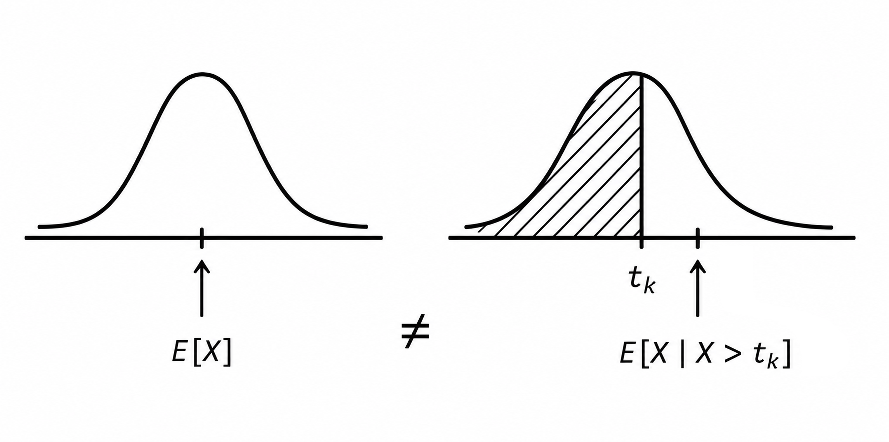
\includegraphics[width=0.8\linewidth]{figures/02_marco_teórico/probabilidad_condicionada.pdf}
    \caption{La duración de una tarea no es, en general, sin memoria. La esperanza incondicional $\mathbb{E}[X]$ (izquierda) difiere de la esperanza condicionada a que la tarea siga en ejecución transcurrido un tiempo $t_k$, $\mathbb{E}[X\mid X>t_k]$ (derecha): el tiempo ya transcurrido desplaza la distribución del tiempo restante.}
    \label{fig:cond-prob}
\end{figure}

El tiempo transcurrido $\delta_e$ es el estadístico suficiente que permite condicionar correctamente la distribución del tiempo restante de cada acción en curso, $F_e$ condicionada al suceso $\{\tau_e>\delta_e\}$, lo que además restaura la propiedad de Markov sobre el estado global. 
 
El SMDP es el caso particular del GSMDP en que a lo sumo un evento está activo en cada instante de decisión. El CTMDP (\textit{Continuous-Time MDP}) es el caso especial en que todos los relojes siguen distribuciones exponenciales: la propiedad de ausencia de memoria de la exponencial hace que el tiempo transcurrido de un reloj activo no aporte información adicional sobre su tiempo restante.
\begin{equation}
    X \sim \textit{Exp}(\lambda) \; \implies \; P(X > t + s \mid X > s) = P(X > t)
\end{equation}

En la práctica, la resolución exacta de un GSMDP con distribuciones generales es computacionalmente intratable; los métodos aproximados recurren a representaciones por fases exponenciales~\cite{younes2004gsmdp} o a planificadores basados en simulación, como MCTS, que muestrean el tiempo de disparo de cada reloj en el evento de finalización (\emph{sample-at-fire}) y no en su inicio, materializando así de forma natural la ausencia de \emph{leak}.

% --------------------------------------------------------------------------- 
\subsection{Procesos de Decisión de Markov Descentralizados} \label{subsec:decposmdp} % ---------------------------------------------------------------------------

Cuando varios agentes deben cooperar para maximizar una recompensa común, pero cada uno solo dispone de observaciones locales y no accede ni al estado global ni a las observaciones de los demás, el modelo apropiado es el \emph{Proceso de Decisión de Markov Descentralizado y Parcialmente Observable} (DEC-POMDP)~\cite{bernstein2002complexity,oliehoek2016concise}.

\begin{definicion}[DEC-POMDP] \label{def:decpomdp} Un DEC-POMDP para $n$ agentes es una tupla \\ $\langle\mathcal{I}, \mathcal{S}, \{\mathcal{A}_i\}, \mathcal{T}, \mathcal{R}, \{\Omega_i\}, \mathcal{O}, \gamma\rangle$ donde: 
\begin{itemize}   
    \item $\mathcal{S}$ es el conjunto de \textbf{estados}.
    \item $\mathcal{I}=\{1,\dots,n\}$ es el conjunto de \textbf{agentes} cooperativos.   
    \item $\{\mathcal{A}_i\}_{1 \leq i \leq n}$ son los conjuntos de acciones locales; la \textbf{acción conjunta} es $\mathbf{a}=(a_1,\dots,a_n)$.   
    \item $\mathcal{T}(s,\mathbf{a},s')$ es la transición sobre el estado global, condicionada a la acción conjunta.   
    \item $\mathcal{R}(s,\mathbf{a})$ es una \textbf{recompensa común} al equipo (agentes plenamente cooperativos).   
    \item $\{\Omega_i\}$ son los conjuntos de observaciones locales. La \textbf{observación conjunta} es \\ $\mathbf{o}=(o_1,\dots,o_n)$.   
    \item $\mathcal{O}(\mathbf{o}\mid s',\mathbf{a})$ es la probabilidad de la observación conjunta. 
    \item $\gamma$ es el factor de descuento.
\end{itemize} 
\end{definicion}

La dificultad esencial es que cada agente debe actuar basándose únicamente en su propia historia de observaciones locales, sin poder construir de forma independiente una creencia sobre el estado global, pues esta depende también de lo que los demás hayan observado y hecho. Esta interdependencia hace que resolver óptimamente un DEC-POMDP de horizonte finito sea estrictamente más difícil que un POMDP de un solo agente~\cite{bernstein2002complexity}. En la práctica, ello obliga a recurrir a métodos aproximados y a estructuras de comunicación explícita que reduzcan la incertidumbre sobre las intenciones ajenas. Esta comunicación se modela dentro del marco formal del DEC-POMDP como acciones locales (agente que envía un mensaje) y como observaciones locales (agente que recibe el mensaje).

El \emph{Proceso de Decisión Semi-Markov Descentralizado y Parcialmente Observable} (DEC-POSMDP) integra en un único modelo la descentralización y la observabilidad parcial del DEC-POMDP con las duraciones continuas del SMDP~\cite{omidshafiei2017decentralized}. Se obtiene intercambiando en la Definición~\ref{def:decpomdp} la función de transición $\mathcal{T}(s,\mathbf{a},s')$ por la \textbf{distribución conjunta de transición y duración} $\mathcal{F}(s',\tau\mid s,\mathbf{a})$ y el factor de descuento discreto $\gamma$ por la \textbf{tasa de descuento continua} $\beta > 0$.
 
Ahora bien, el DEC-POSMDP hereda del SMDP la misma limitación discutida en la Sección~\ref{subsec:gsmdp}: postula directamente la distribución $\mathcal{F}$ y no modela de forma explícita el solapamiento de acciones de duración continua mediante un mecanismo de eventos. Del mismo modo que el GSMDP extiende al SMDP, podemos extender el DEC-POSMDP incorporando la lógica de eventos del GSMP, dando lugar a lo que en este trabajo denominamos \emph{Proceso de Decisión Semi-Markov Generalizado Descentralizado y Parcialmente Observable} (DEC-POGSMDP).
 
\begin{definicion}[DEC-POGSMDP] \label{def:decpogsmdp} Un DEC-POGSMDP para $n$ agentes es la tupla \\ $\langle\mathcal{I}, \mathcal{S}, \{\mathcal{A}_i\}, \mathcal{F}, \mathcal{E}, \mathcal{R}, \{\Omega_i\}, \mathcal{O}, \beta\rangle$, que incorpora a un DEC-POSMDP el mecanismo de eventos del GSMP (Definición~\ref{def:gsmdp}):
\begin{itemize}
    \item $\mathcal{E}$ es el conjunto de \textbf{eventos}. En cada estado $s$, un subconjunto $\mathcal{E}(s)\subseteq\mathcal{E}$ está activo y contiene las finalizaciones de las acciones de duración continua que los agentes tienen en curso. A cada evento activo $e$ se le asocia un \textbf{reloj oculto} $\tau_e\sim F_e$, muestreado en su activación; el evento cuyo reloj expira primero desencadena la transición y el avance del reloj global.
    \item Los relojes son \textbf{latentes}: ninguna observación $o_i$ contiene el valor de un reloj. Cada agente observa únicamente las componentes discretas de su estado y el tiempo transcurrido $\delta_e$ de sus propias acciones en curso.
\end{itemize}
\end{definicion}

La función de utilidad resultante es:
\begin{equation} \label{eq:bellman-decpogsmdp} 
U_\pi(s)=\mathbb{E}_{s',\tau}\!\left[\,\mathcal{R}(s,\pi(s)) +e^{-\beta\tau}\,U_\pi(s')\,\middle|\,s,\pi(s)\right].
\end{equation}
 
No hemos encontrado en la literatura una definición formal de este modelo bajo este nombre; lo introducimos como la progresión natural que resulta de añadir la lógica de eventos del GSMP (Sección~\ref{subsec:gsmdp}) a un DEC-POSMDP. El cambio es conceptualmente menor (reutiliza íntegramente el mecanismo de eventos ya definido para el GSMP) pero metodológicamente importante, pues es lo que garantiza que el modelo trate correctamente las duraciones continuas concurrentes.
 
El DEC-POGSMDP forma el marco teórico que captura todas las características del problema MRTAU distribuido: cooperación de múltiples robots (descentralización), desconocimiento del estado de los compañeros (observabilidad parcial), duraciones continuas y estocásticas modeladas mediante eventos con relojes ocultos (semi-Markov generalizado) e incertidumbre en el éxito de las tareas. La Sección~\ref{sec:formalizacion} desarrolla esta correspondencia.

% =========================================================================== 
\section{El problema MRTAU distribuido como DEC-POGSMDP} \label{sec:formalizacion} % ===========================================================================
 
Con el problema definido en la Sección~\ref{sec:definicion} y los modelos presentados en la Sección~\ref{sec:modelos}, falta enlazar ambas piezas: formalizar el problema como una instancia de la familia de procesos de Markov. Se procede de forma incremental, añadiendo una hipótesis cada vez, hasta llegar al modelo definitivo. La Tabla~\ref{tab:progresion} resume esta progresión.
 
\begin{table}[t] 
    \centering 
    \caption{Progresión de modelos según las hipótesis del problema.} \label{tab:progresion} 
    \begin{tabular}{lccc} 
    \hline \textbf{Variante} & \textbf{Tiempo} & \textbf{Incertidumbre} & \textbf{Observabilidad} \\ 
    \hline MRTA (MDP)     & discreto & no & global 
    \\ MRTAU (GSMDP)   & continuo & sí & global 
    \\ DEC-MRTAU (DEC-POGSMDP) & continuo & sí & local + comunicación 
    \\ \hline 
    \end{tabular} 
\end{table}
 
Las características estáticas de la instancia (Definición~\ref{def:instancia}) (como las ubicaciones, ventanas de ejecución, tabla de capacidades, las recompensas) se consideran parámetros conocidos del modelo. Lo que los siguientes apartados formalizan es la parte dinámica: los estados que evolucionan, las acciones que los modifican y la información disponible en cada decisión.


% --------------------------------------------------------------------------- 
\subsection{MRTA como MDP} \label{subsec:mrta-mdp} % ---------------------------------------------------------------------------

Considérese primero la versión determinista y con observabilidad total: un único planificador centralizado, conocimiento perfecto del estado de robots y tareas, transiciones deterministas y tiempo discretizado. Bajo estas hipótesis, el problema se modela como un MDP (Definición~\ref{def:mdp}).

\begin{itemize}   
    \item \textbf{Estado ($\mathcal{S}$).} El estado global agrega el estado dinámico de robots y tareas junto con el instante de tiempo actual:
    \begin{equation} 
    s=\big(t,\,s^{R_1},\dots,s^{R_n},\,s^{T_1},\dots,s^{T_m}\big) 
    \end{equation} 

    \begin{itemize}
        \item $t$ representa el reloj global, es necesario para comprobar las ventanas de ejecución.
        \item Las variables $s^{R_i},\ 1 \le i \le n$ codifican los estados internos de cada robot. Cada estado contiene la información de:
        \begin{equation}
           s^{R_i}=(x_i,\,b_i,\,j,\,t^{\mathrm{ini}}_i,\,\mathit{op}_i) 
        \end{equation}
        \begin{itemize}
            \item $x_i$ contiene la posición actual del robot.
            \item $b_i \in \mathbb{R}$ contiene el nivel de batería actual del robot.
            \item $j \in \{1 \dots m\} \cup \{0\} $ es un identificador hacia la tarea a la que el robot está actualmente asignado, $j = 0$ en caso de que no esté asignado a ninguna.
            \item $t^{\mathrm{ini}}_i \in \mathbb{R}$ es el instante de tiempo en que el robot inició su acción actual. Junto con el reloj global $t$, permite obtener el tiempo transcurrido $\delta_i = t - t^{\mathrm{ini}}_i$ de la acción en curso. En la versión determinista esta distinción es meramente formal; su relevancia completa se hace explícita al introducir la incertidumbre en la Sección~\ref{subsec:mrtau-gsmdp}.
            \item $\textit{op}_i \in  \{\textsc{Available}, \textsc{Waiting}, \textsc{Executing}, \textsc{Finished} \}$ incluye el estado operativo actual del robot. 
        \end{itemize}
        \item Las variables $s^{T_j},\ 1 \le j \le m$ codifican los estados internos actuales de cada tarea. $s^{T_j} \in  \{\textsc{Pending}, \textsc{Assigned}, \textsc{Executing}, \textsc{Completed} \}$.
        
    \end{itemize}

    \item \textbf{Acciones ($\mathcal{A}$).} Cuando un robot queda libre, es necesario que tome una nueva decisión: Ejecutar una nueva tarea, recargar en la estación de recarga más cercana o terminar (desplazarse a la estación de recarga más cercana y no ejecutar más acciones). Esto define al espacio de acciones:
    \begin{equation}
        \mathcal{A} = \{\textsc{ExecuteTask}(R_i,T_j), \textsc{Recharge}(R_i), \textsc{Finish}(R_i)\}
    \end{equation} 
    
    \item \textbf{Transición ($\mathcal{T}$).} En la versión determinista, $\mathcal{T}(s,a,s')\in\{0,1\}$: ejecutar una tarea (con su coalición completa, dentro de su ventana) la marca como \textsc{Completed} con certeza, desplaza a los robots y consume una cantidad de batería conocida. Esta función de transición se encarga de modelar solamente las transiciones entre los estados de una manera coherente con el problema, respetando las propiedades de una solución (Definición~\ref{def:solucion}).
    
    \item \textbf{Recompensa ($\mathcal{R}$).} Refleja la función objetivo de la Ecuación~\eqref{eq:objetivo}: premia tareas completadas y robots que sobreviven, y penaliza tiempo transcurrido y tareas pendientes. La penalización de tareas pendientes no se aplica hasta alcanzar un estado final. Consideramos una misma recompensa para todas las tareas resueltas, es por eso que la puntuación otorgada a un espisodio completo $\xi$ debe ser:
    \begin{equation}
    \mathcal{R}(\xi) \;=\; \lambda_c\, |\mathcal{T}_{\mathrm{comp}}| \;-\; \lambda_p\, |\mathcal{T}_{\mathrm{pend}}|   \;+\; \lambda_s\, n_{\mathrm{surv}}     \;-\; \lambda_t\, C_{\max}, 
    \end{equation} 
    donde $\mathcal{T}_{\mathrm{comp}}$ y $\mathcal{T}_{\mathrm{pend}}$ son los conjuntos de tareas completadas y pendientes, $n_{\mathrm{surv}}$ es el número de robots que finalizan sin agotar su batería, $C_{\max}$ es el \textit{makespan} y $\lambda_c,\lambda_s,\lambda_t,\lambda_p\ge 0$ ponderan los distintos objetivos, con $\lambda_c+\lambda_s+\lambda_t+\lambda_p = 1$.

    \item \textbf{Factor de descuento ($\gamma = 1$).} Cualquier $\gamma < 1$ descontaría la recompensa terminal en función de la longitud del episodio, lo que distorsionaría artificialmente el objetivo: dos políticas que completen las mismas tareas obtendrían valores distintos según hayan tardado más o menos pasos, y esa penalización por tiempo ya está explícita en la función de recompensa.
\end{itemize}

Este modelo es un punto de partida conceptual y la base de los \textit{baselines} deterministas, pero incurre en dos simplificaciones que lo alejan del problema real (Sección~\ref{subsec:mrtau}): ignora que las duraciones son continuas y estocásticas, y que el éxito de una tarea no está garantizado.

% --------------------------------------------------------------------------- 
\subsection{MRTAU como GSMDP} \label{subsec:mrtau-gsmdp} % ---------------------------------------------------------------------------
 
Al reintroducir las fuentes de incertidumbre de la Sección~\ref{subsec:mrtau}, es necesario aplicar un cambio de modelo. El MDP puede absorber la incertidumbre en el resultado de las tareas, pero no las duraciones continuas y estocásticas. Las tareas pueden ahora fracasar, por lo que se añade el estado \textsc{Failed} al conjunto de estados de tarea, y los robots pueden agotar su batería debido a la variabilidad de los tiempos, por lo que se añade igualmente el estado operativo \textsc{Failed}.
 
Manteniendo todavía la hipótesis de observabilidad global, podría pensarse en modelar esta variante como un SMDP, sustituyendo la transición discreta por la distribución conjunta de transición y duración $\mathcal{F}(s',\tau\mid s,a)$. Sin embargo, como se estableció en la Sección~\ref{subsec:gsmdp}, hacerlo provocaría inevitablemente el \emph{leak temporal} (Figura~\ref{fig:leak}): bajo observabilidad total, fijar la duración de una tarea en el instante en que comienza expondría su instante de finalización a cualquier robot que decida antes de que termine. La variante MRTAU debe modelarse, por tanto, como un \textbf{GSMDP} (Definición~\ref{def:gsmdp}), tratando cada ejecución en curso como un evento con un reloj oculto.
 
\paragraph{La cola de eventos.} La dinámica se articula mediante una cola de eventos. Cada acción no determinista de duración continua (ejecución de tareas) programa en la cola un evento de finalización con su instante de disparo (el valor de su reloj). El sistema avanza saltando de evento en evento: en cada paso se extrae de la cola el evento con menor instante de disparo, se avanza el reloj global $t$ hasta él, se actualiza el estado correspondiente (la tarea pasa a \textsc{Completed} o \textsc{Failed}, el robot a \textsc{Available}, etc.) y, si la transición deja a algún robot libre, se le solicita una nueva decisión. Los instantes de disparo permanecen en la cola, internos al modelo, pero nunca forman parte del estado que la política observa: es esta ocultación la que elimina el \emph{leak}.
 
\paragraph{Resultado y duración desconocidos hasta la finalización.} La consecuencia central de este mecanismo es que, al iniciar una acción $\textsc{ExecuteTask}(T_j)$, \emph{no se conoce ni cuánto durará la ejecución ni si tendrá éxito}. El reloj del evento de finalización codifica ambos resultados, que permanecen ocultos hasta que el evento se dispara. Solo en el instante de finalización se revela el desenlace: éxito con probabilidad $\rho_j$ y duración muestreada de $\mathcal{N}(\mu_t^s,\sigma_t^s)$, o fracaso con probabilidad $1-\rho_j$ y duración de $\mathcal{N}(\mu_t^f,\sigma_t^f)$. Hasta ese momento, el estado solo refleja que la tarea está \textsc{Executing} y, a través del instante de inicio $t^{\mathrm{ini}}_i$ almacenado en el estado del robot (Sección~\ref{subsec:mrta-mdp}), cuánto tiempo lleva en ejecución. Este tiempo transcurrido $\delta_i = t - t^{\mathrm{ini}}_i$ es información del pasado, legítimamente observable, y es además el estadístico suficiente que permite condicionar correctamente la distribución del tiempo restante mediante $F\mid\{\tau>\delta_i\}$ (Figura~\ref{fig:cond-prob}).
 
Así modelada, la variante MRTAU es un GSMDP completamente observable. La principal consecuencia es que la solución óptima ya no es una asignación fija calculada \textit{a priori}, sino una política adaptativa que responde a los resultados observados a medida que los eventos se disparan; esto justifica el empleo de algoritmos \textit{online}. No obstante, este modelo aún conserva una hipótesis fuerte: la observabilidad global, coherente solo con una arquitectura centralizada.


% --------------------------------------------------------------------------- 
\subsection{DEC-MRTAU como DEC-POGSMDP} \label{subsec:decmrtau-decpogsmdp} % ---------------------------------------------------------------------------
 
El núcleo de este trabajo consiste en eliminar la última hipótesis: la observabilidad global. En un sistema verdaderamente distribuido no existe coordinador ni estado compartido; cada robot decide de forma autónoma a partir de su información local. Esta relajación transforma el GSMDP en un DEC-POGSMDP (Sección~\ref{subsec:decposmdp}), dando lugar a la variante \emph{DEC-MRTAU}, modelo formal definitivo del problema, definido por la tupla \begin{equation} \label{eq:tupla-decpogsmdp} \big\langle\,\mathcal{I},\mathcal{S},\{\mathcal{A}_i\}, \mathcal{F}, \mathcal{E},\mathcal{R}, \{\Omega_i\},\mathcal{O}\,\big\rangle, \end{equation} cuyos elementos se concretan a continuación.
 
\paragraph{Agentes ($\mathcal{I}$).} El conjunto de $n$ robots cooperativos. Comparten un único objetivo de equipo, por lo que el problema es plenamente cooperativo.
 
\paragraph{Estado global ($\mathcal{S}$).} Idéntico al de las variantes anteriores, $s=(t,s^{R_1},\dots,s^{R_n},s^{T_1},\dots,s^{T_m})$. La diferencia esencial es que este estado global ningún agente lo observa por completo: existe en el modelo, pero no en la percepción de los robots.
 
\paragraph{Acciones ($\{\mathcal{A}_i\}_{1 \leq i \leq n}$).} Cada robot dispone de sus acciones locales $\{ \textsc{ExecuteTask}(T_j), \\ \textsc{Recharge}, \textsc{Finish} \}$. Adicionalmente, según el algoritmo de coordinación, los robots realizan acciones de comunicación (difundir una puja, una distribución sobre sus planes, etc.) que no modifican el entorno físico pero condicionan las decisiones de los demás. Las tareas \textit{multi-robot} ($q_j>1$) son aquí especialmente delicadas, pues exigen acordar coaliciones sin observabilidad mutua, lo que solo puede lograrse mediante la comunicación.

\paragraph{Transiciones y Duraciones ($\mathcal{F}$).} Dinámica semi-Markoviana generalizada con duraciones continuas estocásticas e incertidumbre en el éxito de las tareas (el componente ``$+U$''), inducida por el mecanismo de eventos y condicionada a la acción conjunta: $\mathcal{F}(s',\tau\mid s,\mathbf{a})$.
 
\paragraph{Eventos ($\mathcal{E}$).} Como en la variante centralizada (Sección~\ref{subsec:mrtau-gsmdp}), las acciones de duración continua generan eventos de finalización con relojes ocultos, gestionados por una cola de eventos; el resultado y la duración de cada tarea solo se revelan al dispararse el evento correspondiente. Es esta componente la que distingue el DEC-POGSMDP de un mero DEC-POSMDP y la que garantiza, también en el caso distribuido, que ningún agente anticipe el desenlace de una ejecución en curso. 

\paragraph{Recompensa ($\mathcal{R}$).} Función global cooperativa (Ecuación~\eqref{eq:objetivo}), común a todos los agentes: maximiza tareas completadas y robots que preservan su integridad, y minimiza tiempo de ejecución y tareas pendientes.
 
\paragraph{Observabilidad ($\{\Omega_i\}_{1 \leq i \leq n}$, $\mathcal{O}$).} Es el elemento que distingue conceptualmente al DEC-MRTAU. El espacio de observaciones de cada robot es la tupla \begin{equation} \label{eq:observacion} o_i=\big(s^{R_i},\,\mathbf{s}^{T},\,\mathcal{M}_{\mathrm{in}}\big), \end{equation} formada por su propio estado, el estado de las tareas y los mensajes recibidos. La función de observación $\mathcal{O}$ actúa como un \emph{filtro de la realidad} con una estructura híbrida característica de este problema: 
\begin{itemize}   
    \item \textbf{Parte totalmente observable.} El robot conoce con exactitud su propio estado $s^{R_i}$ ---batería, ubicación, disponibilidad y, en particular, el tiempo transcurrido $\delta_i$ de su propia acción en curso--- y el estado de todas las tareas $\mathbf{s}^{T}$. Sobre esta parte el modelo se comporta de forma observable, y sobre ella cada robot condiciona correctamente la finalización de su propia ejecución.   
    \item \textbf{Parte oculta.} El robot desconoce el estado interno y la ubicación de los demás robots, $s^{R_{k}}, k \neq i$: no sabe dónde están sus compañeros, cuánta batería les queda ni qué tarea pretenden ejecutar; tampoco, por tanto, los relojes de sus acciones. Es esta componente la que introduce la observabilidad parcial y sitúa el problema en el marco DEC-POGSMDP en lugar del GSMDP. 
\end{itemize}
Obsérvese que esta estructura refuerza la ausencia de \emph{leak temporal}: si en el modelo centralizado había que ocultar deliberadamente los relojes para evitar la fuga, aquí la imposibilidad de observar a los compañeros la convierte en estructural (un robot no puede ``ver el futuro'' de otro porque no puede observar a ese otro en absoluto). La lógica de eventos del DEC-POGSMDP sigue siendo necesaria, no obstante, para tratar correctamente la propia ejecución de cada robot, cuyo desenlace tampoco debe conocerse por anticipado.
 
\paragraph{El papel de la comunicación.} La incertidumbre sobre las intenciones ajenas (en particular, el riesgo de que dos robots seleccionen la misma tarea o de que no se forme la coalición requerida) no puede eliminarse mediante observación directa, pero sí mitigarse mediante el intercambio explícito de mensajes $\mathcal{M}_{\mathrm{in}}$. La comunicación es, por tanto, el mecanismo que sustituye a la observabilidad global ausente: en lugar de ver el estado de los compañeros, cada robot infiere parcialmente sus intenciones a partir de lo que estos comunican. Bajo este prisma, los distintos algoritmos analizados en este trabajo (desde los \textit{baselines} sin comunicación hasta los métodos de pujas CBAA/CBBA y la planificación distribuida Dec-MCTS) pueden entenderse como diferentes políticas de comunicación que resuelven el mismo DEC-POGSMDP con grados crecientes de coordinación. Esta lectura unificada permite comparar de forma directa la planificación distribuida con el MCTS centralizado del modelo base \red{CITA AL TUTOR}.
 
En síntesis, la transición desde un planteamiento centralizado (MDP/GSMDP con observabilidad global) a uno puramente distribuido (DEC-POGSMDP) no es una mera elección de implementación, sino una reformulación que cambia la clase de complejidad del problema y obliga a sustituir la información global por mecanismos de coordinación basados en comunicación. Es esta reformulación la que define la contribución principal del trabajo.


% ===========================================================================
\section{Algoritmos propuestos} \label{sec:algoritmos}
% ===========================================================================

Con la única excepción de la variante más elemental de MRTA (ST-SR-IA), el resto de variantes de MRTA, y en particular el problema MRTAU abordado en este trabajo, son NP-duras~\cite{gerkey2004taxonomy}. En consecuencia, salvo en instancias triviales, no es realista aspirar a hallar la solución óptima. Esta dificultad se agrava al introducir la incertidumbre (Sección~\ref{subsec:mrtau}): cuando las ejecuciones son estocásticas, la solución deja de ser una asignación fija y pasa a ser una política que debe adaptarse al estado observado en cada instante (Sección~\ref{subsec:decmrtau-decpogsmdp}). Los algoritmos no persiguen, por tanto, la optimalidad, sino soluciones suficientemente buenas obtenidas con un coste de cómputo y de comunicación asumible.
 
En el problema distribuido, la comunicación desempeña un papel central en esa búsqueda: es el mecanismo que sustituye la observabilidad global ausente y permite a los robots coordinar sus decisiones (Sección~\ref{subsec:decmrtau-decpogsmdp}). Ahora bien, la comunicación no puede suponerse ilimitada. Definir una comunicación perfecta y sin coste, en la que cada robot difundiera de forma continua su estado completo al resto, cancelaría por completo el sentido del planteamiento descentralizado: cada agente podría reconstruir el estado global y el problema colapsaría de nuevo en uno centralizado, contradiciendo las propias motivaciones (robustez, escalabilidad y tolerancia a comunicación limitada o intermitente) que justifican el enfoque distribuido (Sección~\ref{subsec:centralizado-descentralizado}). El interés reside, precisamente, en alcanzar buenas soluciones intercambiando una cantidad de información acotada.
 
Bajo este prisma, los algoritmos considerados pueden leerse de forma unificada como distintas \textbf{políticas de comunicación} que resuelven el mismo DEC-POGSMDP con grados crecientes de coordinación: desde la ausencia total de comunicación (\textit{baselines}, Sección~\ref{subsec:baselines}), pasando por la negociación de coaliciones mediante pujas (CBAA y CBBA, Sección~\ref{subsec:pujas}), hasta la planificación distribuida que comunica distribuciones sobre los planes (Dec-MCTS, Sección~\ref{subsec:dec-mcts}). Todos comparten la naturaleza \textit{online} y reactiva justificada en la Sección~\ref{subsec:online-offline}: se invocan en cada instante de decisión y devuelven una única acción. La política global emerge de la invocación repetida del procedimiento conforme avanza la cola de eventos.

% ---------------------------------------------------------------------------
\subsection{\textit{Baselines}: Greedy y Random} \label{subsec:baselines}
% ---------------------------------------------------------------------------

Los dos \textit{baselines} constituyen las referencias frente a las que se medirá la aportación del resto de algoritmos. Su rasgo definitorio es la \textbf{ausencia de comunicación}: cada robot decide exclusivamente a partir de su propio estado $s^{R_i}$ y del estado de las tareas $\mathbf{s}^{T}$, ignorando por completo a los demás robots (el conjunto de mensajes $\mathcal{M}_{\mathrm{in}}$ de la observación~\eqref{eq:observacion} permanece vacío). En términos del DEC-POGSMDP representan la política de comunicación degenerada y se comportan como si cada robot resolviera un MDP puramente local.

Como consecuencia de falta de comunicación, los \textit{baselines} carecen de coordinación (no razonan sobre las coaliciones $q_j$ ni sobre los conflictos con otros robots) y no trabajan con la incertidumbre (no emplean la probabilidad de éxito $\rho_j$ ni las distribuciones de duración). La única condición de factibilidad que comprueban es la energética: una tarea $T_j$ se considera \emph{alcanzable} si el robot dispone de batería suficiente para desplazarse hasta ella:
\begin{equation} \label{eq:alcanzable}
    \mathrm{coste}_{ij} \;=\; \frac{d(x_i, x_j)}{v_i}\,\cdot\,\textit{rate-}R_i \;\le\; b_i .
\end{equation}

Ambos algoritmos comparten el mismo esqueleto de decisión y se diferencian únicamente en el criterio de selección de tarea. El esqueleto distingue tres situaciones: si no quedan tareas pendientes en el escenario, el robot ha terminado su cometido y emite \textsc{Finish}; si quedan tareas pendientes pero ninguna es alcanzable con la batería actual, la mejor opción es \textsc{Recharge} y reintentar más tarde; en otro caso, el robot selecciona una de las tareas alcanzables y la ejecuta. El \textbf{Random} (Algoritmo~\ref{alg:random}) elige una tarea alcanzable de manera aleatoria, conforma el peor escenario de coordinación posible. El \textbf{Greedy} (Algoritmo~\ref{alg:greedy}) elige la tarea alcanzable más cercana según la función de distancia $d(\cdot,\cdot)$, introduciendo una heurística mínima de eficiencia, pero sin ninguna anticipación de conflictos.

\begin{algorithm}
\caption{\textsc{Random} --- decisión de $R_i$ en un instante de decisión}
\label{alg:random}
\begin{algorithmic}[1]
\Require observación $o_i=(s^{R_i},\mathbf{s}^{T},\mathcal{M}_{\mathrm{in}})$
\Ensure acción local
\State $\mathcal{P} \gets \{\,T_j \in \mathcal{T} : s^{T_j}=\textsc{Pending}\,\}$ \Comment{tareas pendientes}
\State $\mathcal{A}_{\mathrm{alc}} \gets \{\,T_j \in \mathcal{P} : \mathrm{coste}_{ij}\le b_i\,\}$ \Comment{alcanzables, Ec.~\eqref{eq:alcanzable}}
\If{$\mathcal{P}=\varnothing$} \Return $\textsc{Finish}$
\ElsIf{$\mathcal{A}_{\mathrm{alc}}=\varnothing$} \Return $\textsc{Recharge}$
\Else
    \State $T_j \gets$ tarea elegida uniformemente al azar de $\mathcal{A}_{\mathrm{alc}}$
    \State \Return $\textsc{ExecuteTask}(T_j)$
\EndIf
\end{algorithmic}
\end{algorithm}

\begin{algorithm}
\caption{\textsc{Greedy} --- decisión de $R_i$ en un instante de decisión}
\label{alg:greedy}
\begin{algorithmic}[1]
\Require observación $o_i=(s^{R_i},\mathbf{s}^{T},\mathcal{M}_{\mathrm{in}})$
\Ensure acción local
\State $\mathcal{P} \gets \{\,T_j \in \mathcal{T} : s^{T_j}=\textsc{Pending}\,\}$
\State $\mathcal{A}_{\mathrm{alc}} \gets \{\,T_j \in \mathcal{P} : \mathrm{coste}_{ij}\le b_i\,\}$ \Comment{Ec.~\eqref{eq:alcanzable}}
\If{$\mathcal{P}=\varnothing$} \Return $\textsc{Finish}$
\ElsIf{$\mathcal{A}_{\mathrm{alc}}=\varnothing$} \Return $\textsc{Recharge}$
\Else
    \State $T_j \gets \arg\min_{T_k\in\mathcal{A}_{\mathrm{alc}}} d(x_i, x_k)$ \Comment{tarea alcanzable más cercana}
    \State \Return $\textsc{ExecuteTask}(T_j)$
\EndIf
\end{algorithmic}
\end{algorithm}


% ---------------------------------------------------------------------------
\subsection{Algoritmos basados en pujas: CBAA y CBBA} \label{subsec:pujas}
% ---------------------------------------------------------------------------

El siguiente paso incorpora la coordinación mediante mecanismos de mercado. El \emph{Consensus-Based Auction Algorithm} (CBAA) y su extensión, el \emph{Consensus-Based Bundle Algorithm} (CBBA), fueron propuestos por Choi, Brunet y How~\cite{choi2009consensus} como métodos descentralizados en los que cada agente puja por las tareas según una función de \emph{score} y los conflictos se resuelven mediante una fase de consenso basada en comunicación local. A diferencia de los \textit{baselines}, aquí los robots intercambian información: difunden sus pujas y reciben las de sus vecinos. Este intercambio se modela mediante las acciones de comunicación del DEC-POGSMDP (Sección~\ref{subsec:decmrtau-decpogsmdp}) y se realiza mediante las funciones \textsc{CommunicateBid} y \textsc{ReceiveBid}, que encapsulan la difusión de pujas y la recepción de las pujas ajenas.

\paragraph{Aproximación determinista del \textit{score}.} Ambos algoritmos adoptan un tratamiento determinista de la incertidumbre que caracteriza a MRTAU. Por un lado, la probabilidad de éxito $\rho_j$ de una tarea se asume conocida y se emplea directamente como peso de su puntuación: las tareas con mayor probabilidad de completarse con éxito reciben un \textit{score} más alto. Por otro, la duración esperada de la ejecución de una tarea se puede calcular combinando de las medias de las distribuciones de éxito $\mathcal{N}(\mu_j^{s},\sigma_j^{s})$ y de fracaso $\mathcal{N}(\mu_j^{f},\sigma_j^{f})$ como:
\begin{equation} \label{eq:duracion-esperada}
    \bar{d}_j \;=\; \rho_j\,\mu_j^{s} \;+\; (1-\rho_j)\,\mu_j^{f},
\end{equation}

En la práctica, esto significa que las pujas se resuelven en cada instante de decisión de manera determinista, haciendo uso de las esperanzas matemáticas de las variables aleatorias probabilidad de éxito y tiempo de ejecución.

Concretamente, para un robot $R_i$ que evalúa la tarea $T_j$ desde una posición de partida en un instante de disponibilidad $t_i^{\mathrm{libre}}$, se estima el tiempo de viaje $\Delta_{ij}^{\mathrm{viaje}}=d(x_i,x_j)/v_i$ y el instante de llegada $t_{ij}^{\mathrm{llegada}}=t_i^{\mathrm{libre}}+\Delta_{ij}^{\mathrm{viaje}}$. Si la llegada excede el límite de la ventana ($t_{ij}^{\mathrm{lleg}}>t_j^{l}$), la puja es nula. En otro caso, considerando el tiempo de espera $\Delta_{ij}^{\mathrm{espera}}=\max(0,\,t_j^{s}-t_{ij}^{\mathrm{llegada}})$ y la duración esperada \eqref{eq:duracion-esperada}, se define la inversión temporal total $\tau_{ij}=\Delta_{ij}^{\mathrm{viaje}}+\Delta_{ij}^{\mathrm{espera}}+\bar{d}_j$ y la puja (\textit{score}) es finalmente:
\begin{equation} \label{eq:puja}
    \nu_{ij}
    \;=\;
    \underbrace{\frac{\rho_j}{1+\tau_{ij}}}_{\text{valor base}}
    \;\cdot\;
    \underbrace{\frac{a_j+1}{q_j}}_{\text{factor de cooperación}} ,
\end{equation}
donde $a_j$ es el número de robots ya asignados a $T_j$ y $q_j$ el número de robots requeridos para la ejecución. El valor base es creciente en la probabilidad de éxito $\rho_j$ y decreciente en el tiempo invertido $\tau_{ij}$, mientras que el factor de cooperación fomenta la formación de coaliciones.

\paragraph{Estimación del instante de disponibilidad.} El cálculo de la puja~\eqref{eq:puja} requiere conocer el instante $t_i^{\mathrm{libre}}$ en que el robot evaluado queda libre y puede emprender el desplazamiento hacia $T_j$. Para el robot que toma la decisión esta información es inmediata: se encuentra en estado \textsc{Available} y su instante de disponibilidad es el reloj global, $t_i^{\mathrm{libre}}=t$. La dificultad surge al evaluar las pujas de los demás robots, pues un robot puede hallarse a mitad de una acción de duración estocástica y su instante de finalización no es conocido. Para resolverlo se emplea una función auxiliar, $\textsc{EstimateNextAvailability}$, que infiere $t_k^{\mathrm{libre}}$ a partir de la situación en que se encuentra el robot $R_k$. Caben cuatro casos:
 
\begin{itemize}
    \item \textbf{Acción de duración determinista.} Si el robot está disponible, desplazándose o recargando, la duración de su acción en curso es conocida (los desplazamientos y las recargas son deterministas en el modelo, al depender solo de distancias, velocidades y tasas de recarga). Su instante de disponibilidad es, por tanto, el instante de finalización ya programado, sin necesidad de estimación.
    \item \textbf{En espera de coalición (tarea \textsc{Pending}).} El robot ha llegado a una tarea, pero la coalición de $q_j$ trabajadores aún no se ha completado, de modo que permanece a la espera de sus compañeros. Como dicha coalición podría no llegar a formarse, se adopta una estimación conservadora: el robot quedará libre, en el peor caso, cuando se agote la ventana de ejecución, esto es, en el instante límite $t_j^{l}$.
    \item \textbf{Coalición completa sin iniciar (tarea \textsc{Assigned}).} La coalición está formada y la ejecución comenzará en un instante conocido, pero todavía no ha empezado. Al no disponer de información sobre el transcurso de la ejecución, la disponibilidad se estima como ese instante de inicio más la duración esperada $\bar{d}_j$ de la Ecuación~\eqref{eq:duracion-esperada}.
    \item \textbf{En ejecución (tarea \textsc{Executing}).} El robot ejecuta la tarea desde un instante de inicio $t^{\mathrm{inicio}}$ y ha transcurrido un tiempo $\delta = t - t^{\mathrm{inicio}}$. Este es el caso no trivial y se desarrolla a continuación.
\end{itemize}
 
El caso de una tarea en ejecución conecta directamente con la discusión del GSMDP (Sección~\ref{subsec:gsmdp}): el tiempo transcurrido $\delta$ es información del pasado, legítimamente observable, y constituye el estadístico suficiente que permite condicionar la distribución del tiempo restante (Figura~\ref{fig:cond-prob}). No puede emplearse la duración esperada incondicional, ya que el hecho de que la tarea siga en curso transcurrido $\delta$ desplaza esa distribución; se busca, en su lugar, la esperanza de la duración total $X$ condicionada al suceso $\{X>\delta\}$, esto es, $\mathbb{E}[X\mid X>\delta]$.
 
A esta dependencia del tiempo transcurrido se añade que la duración no obedece a una única distribución, sino a una combinación de dos componentes, ya que el desenlace de la tarea permanece desconocido hasta su finalización (Sección~\ref{subsec:mrtau-gsmdp}): con probabilidad \textit{a priori} $\rho_j$ la tarea concluirá con éxito y su duración se distribuye según $\mathcal{N}(\mu_j^{s},\sigma_j^{s})$, mientras que con probabilidad $1-\rho_j$ fracasará con duración $\mathcal{N}(\mu_j^{f},\sigma_j^{f})$ de modo que
\begin{equation}
    X \sim \rho_j \cdot  \mathcal{N}(\mu_j^{s},\sigma_j^{s}) \;\ + \;\ (1-\rho_j) \cdot  \mathcal{N}(\mu_j^{f},\sigma_j^{f})
\end{equation}
Observar que la tarea no ha terminado ($X>\delta$) aporta información no solo sobre el tiempo restante, sino también sobre cuál de los dos desenlaces es más probable. El cálculo procede, en consecuencia, en dos etapas.
 
\emph{Primera etapa: actualización bayesiana del desenlace.} Sea $\phi$ la función de densidad de la distribución normal y sea $\Phi$ su función de distribución acumulada ($\Phi(z) = P(Z \le z)$), la probabilidad de que cada componente supere el tiempo transcurrido es respectivamente ($1-\Phi(z_s)$) y ($1-\Phi(z_f)$), con $z_s=(\delta-\mu_j^{s})/\sigma_j^{s}$ y $z_f=(\delta-\mu_j^{f})/\sigma_j^{f}$. La probabilidad marginal de que una tarea supere el tiempo transcurrido es
\begin{equation} \label{eq:surv-marginal}
    P(X>\delta) \;=\; \rho_j\,(1-\Phi(z_s)) \;+\; (1-\rho_j)\, (1-\Phi(z_f)).
\end{equation}
El teorema de Bayes proporciona entonces la probabilidad \emph{a posteriori} de que la ejecución acabe en éxito, dado que sigue en curso,
\begin{equation} \label{eq:posterior-success}
    P(S\mid X>\delta) \;=\; \frac{P(S)\,P(X>\delta\mid S)}{P(X>\delta)}
    \;=\; \frac{\rho_j\,\bigl(1-\Phi(z_s)\bigr)}{\rho_j\,\bigl(1-\Phi(z_s)\bigr) + (1-\rho_j)\,\bigl(1-\Phi(z_f)\bigr)},
\end{equation}
y, de forma análoga, la probabilidad a posteriori de fracaso,
\begin{equation} \label{eq:posterior-fail}
    P(F\mid X>\delta) \;=\; \frac{(1-\rho_j)\,\bigl(1-\Phi(z_f)\bigr)}{\rho_j\,\bigl(1-\Phi(z_s)\bigr) + (1-\rho_j)\,\bigl(1-\Phi(z_f)\bigr)}.
\end{equation}
Intuitivamente, si las ejecuciones fallidas tienden a prolongarse, una tarea que se demora ve incrementada su probabilidad a posteriori de fracaso.
 
\emph{Segunda etapa: esperanza condicionada por componente.} Condicionada a cada desenlace, la duración sigue una normal truncada por la izquierda en $\delta$. Para el desenlace de éxito, su función de densidad es
\begin{equation} \label{eq:trunc-density}
    f_{X_s\mid X_s>\delta}(x) \;=\; \frac{f_{X_s}(x)}{P(X_s>\delta)}\,\mathbf{1}_{(\delta,\,+\infty)}(x),
\end{equation}
donde $\mathbf{1}_{(\delta,+\infty)}$ es la función indicatriz. Sustituyendo la densidad normal $f_{X_s}(x)=\tfrac{1}{\sigma_j^{s}}\,\phi\!\bigl((x-\mu_j^{s})/\sigma_j^{s}\bigr)$ y $P(X_s>\delta)=1-\Phi(z_s)$, la esperanza condicionada se expresa como
\begin{equation} \label{eq:integrals-conditional}
    \mathbb{E}[X\mid X>\delta, S]
    \;=\; \int_{\delta}^{+\infty} x \, \frac{f_{X_s}(x)}{P(X_s>\delta)} \, dx
    \;=\; \frac{1}{1-\Phi(z_s)} \int_{\delta}^{+\infty} \frac{x}{\sigma_j^{s}}\,\phi\!\left(\frac{x-\mu_j^{s}}{\sigma_j^{s}}\right) dx.
\end{equation}
El cambio de variable $z=(x-\mu_j^{s})/\sigma_j^{s}$, que implica $x=\mu_j^{s}+\sigma_j^{s}\,z$ y $dx=\sigma_j^{s}\,dz$, transforma esta integral en
\begin{equation} \label{eq:integrals2-conditional}
\begin{split}
    \mathbb{E}[X\mid X>\delta, S]
    &= \frac{1}{1-\Phi(z_s)} \int_{z_s}^{+\infty} \bigl(\mu_j^{s}+\sigma_j^{s}\,z\bigr)\,\phi(z)\,dz \\[6pt]
    &= \frac{\mu_j^{s}}{1-\Phi(z_s)} \int_{z_s}^{+\infty} \phi(z)\,dz
       \;+\; \frac{\sigma_j^{s}}{1-\Phi(z_s)} \int_{z_s}^{+\infty} z\,\phi(z)\,dz \\[6pt]
    &= \frac{1-\Phi(z_s)}{1-\Phi(z_s)}\,\mu_j^{s}
       \;+\; \frac{\sigma_j^{s}}{1-\Phi(z_s)}\,\bigl[-\phi(z)\bigr]_{z_s}^{+\infty} \\[6pt]
    &= \mu_j^{s} \;+\; \sigma_j^{s}\,\frac{\phi(z_s)}{1-\Phi(z_s)},
\end{split}
\end{equation}
donde se han empleado las identidades $\Phi'(z)=\phi(z)$ y $\phi'(z)=-z\,\phi(z)$ para resolver la primera y la segunda integral, respectivamente. Procediendo de manera idéntica para el desenlace de fracaso se llega a
\begin{equation} \label{eq:integrals3-conditional}
    \mathbb{E}[X\mid X>\delta, F] \;=\; \mu_j^{f} \;+\; \sigma_j^{f}\,\frac{\phi(z_f)}{1-\Phi(z_f)}.
\end{equation}

Combinando ambas etapas, se tiene entonces la esperanza condicionada de la duración total,
\begin{equation} \label{eq:cond-exp}
    \mathbb{E}[X\mid X>\delta] \;=\; \mathbb{E}[X\mid X>\delta, S] \, P(S \mid X>\delta) \;+\; \mathbb{E}[X\mid X>\delta, F] \, P(F\mid X>\delta).
\end{equation}
El instante de disponibilidad estimado del robot se obtiene finalmente sumando esta duración al instante de inicio de la tarea,
\begin{equation} \label{eq:freetime}
    t_k^{\mathrm{libre}} \;=\; t^{\mathrm{inicio}} + \mathbb{E}[X\mid X>\delta],
\end{equation}
valor que luego se emplea en el cálculo de los tiempos de viaje, espera y, en última instancia, la puja $\nu_{ij}$ de la Ecuación~\eqref{eq:puja}. Conviene subrayar que esta estimación es una aproximación determinista coherente con el resto del \textit{score} (se resume la distribución del tiempo restante en su esperanza), y que reproduce a nivel de planificación el mismo condicionamiento por tiempo transcurrido que el modelo de eventos del GSMDP realiza de forma exacta.

\paragraph{CBAA: subasta de tarea individual.} En el CBAA (Algoritmo~\ref{alg:cbaa}), cada robot evalúa todas las tareas alcanzables, las ordena por puja decreciente y recorre esa lista de preferencias. Para cada tarea candidata $T_j$, recaba mediante \textsc{CommunicateBid} las pujas de los vecinos que compiten por ella y cuenta cuántos la superan. La tarea dispone de $q_j-a_j$ plazas libres; el robot se adjudica una plaza (y emite $\textsc{ExecuteTask}(T_j)$) si y solo si figura entre los mejores postores que caben en esas plazas, es decir, si el número de pujas superiores es estrictamente menor que el de plazas disponibles. Si pierde el consenso en su tarea preferida, pasa a la siguiente; si agota la lista sin éxito, recarga o termina según queden o no tareas inalcanzables por batería.

\begin{algorithm}
\caption{\textsc{CBAA} --- decisión de $R_i$ en un instante de decisión}
\label{alg:cbaa}
\begin{algorithmic}[1]
\Require observación $o_i=(s^{R_i},\mathbf{s}^{T},\mathcal{M}_{\mathrm{in}})$
\Ensure acción local
\State $\mathcal{P} \gets \{\,T_j : s^{T_j}=\textsc{Pending}\,\}$
\If{$\mathcal{P}=\varnothing$} \Return $\textsc{Finish}$ \EndIf
\State para cada $T_j\in\mathcal{P}$ alcanzable: calcular $\nu_{ij}$ según~\eqref{eq:puja}
\State ordenar las tareas con $\nu_{ij}>0$ por puja decreciente
\For{$T_j$ en orden de preferencia}
    \State \textsc{ComunicateBid}$(\nu_{ij})$
    \State $\{\nu_{kj}\}_{k\neq i} \gets$ \textsc{ReceiveBid}() \Comment{pujas de los vecinos por $T_j$}
    \State $n_{\mathrm{sup}} \gets \big|\{\,k\neq i : \nu_{kj}>\nu_{ij}\,\}\big|$ \Comment{vecinos que nos superan}
    \State $\text{plazas} \gets q_j - a_j$
    \If{$\text{plazas}>0$ \textbf{y} $n_{\mathrm{sup}}<\text{plazas}$}
        \State \Return $\textsc{ExecuteTask}(T_j)$ \Comment{entramos entre los mejores postores}
    \EndIf
\EndFor
\If{queda alguna tarea pendiente inalcanzable por batería} \Return $\textsc{Recharge}$
\Else{} \Return $\textsc{Finish}$ \EndIf
\end{algorithmic}
\end{algorithm}

\paragraph{CBBA: construcción de paquetes.} El CBBA (Algoritmo~\ref{alg:cbba}) generaliza el anterior planificando secuencias de tareas. Cada robot construye de forma voraz un paquete (\textit{bundle}): partiendo de su estado, añade iterativamente la tarea de mayor puja marginal~\eqref{eq:puja}, recalculada desde un estado virtual que actualiza la posición, el reloj y la batería de manera estocástica como si las tareas ya incorporadas se hubieran ejecutado (procedimiento \textsc{BuildBestBundle}). El proceso se detiene al alcanzar un tamaño máximo de paquete, al agotar la batería virtual o al no quedar tareas alcanzables. Pese a planificar secuencias a largo plazo, el robot solo compromete la primera tarea del paquete; el resto actúa como anticipación (\textit{lookahead}) que informa la puja. La resolución de conflictos compara, sobre esa primera tarea, las pujas marginales de los vecinos cuyos paquetes la contienen: si el robot no es superado en más plazas de las disponibles, la ejecuta; en otro caso la elimina de la lista de tareas disponibles y reconstruye el paquete, repitiendo la negociación.

\begin{algorithm}
\caption{\textsc{CBBA} --- decisión de $R_i$ en un instante de decisión}
\label{alg:cbba}
\begin{algorithmic}[1]
\Require observación $o_i=(s^{R_i},\mathbf{s}^{T},\mathcal{M}_{\mathrm{in}})$
\Ensure acción local
\State $\mathcal{P} \gets \{\,T_j : s^{T_j}=\textsc{Pending}\,\}$
\If{$\mathcal{P}=\varnothing$} \Return $\textsc{Finish}$ \EndIf
\State $\mathcal{N} \gets \varnothing$ \Comment{lista negra de tareas perdidas}
\While{\textbf{True}}
    \State $\mathcal{B} \gets \textsc{BuildBestBundle}(R_i, \mathcal{N})$
    \If{$\mathcal{B}=\varnothing$}
        \State \Return $\textsc{Recharge}$ si hay tareas inalcanzables, en otro caso $\textsc{Finish}$
    \EndIf
    \State $T^{*} \gets$ primera tarea de $\mathcal{B}$; \quad $\nu^{*} \gets$ puja marginal de $T^{*}$
    \State \textsc{CommunicateBundleBid}(paquete $\mathcal{B}$ y sus pujas)
    \State $\{\mathcal{B}_k\}_{k\neq i} \gets$ \textsc{ReceiveBundleBid}() \Comment{paquetes de los vecinos}
    \State $n_{\mathrm{sup}} \gets \big|\{\,k\neq i : T^{*}\in\mathcal{B}_k \text{ con puja marginal} > \nu^{*}\,\}\big|$
    \State $\text{plazas} \gets q_{T^{*}} - a_{T^{*}}$
    \If{$\text{plazas}>0$ \textbf{y} $n_{\mathrm{sup}}<\text{plazas}$}
        \State \Return $\textsc{ExecuteTask}(T^{*})$
    \Else
        \State $\mathcal{N} \gets \mathcal{N}\cup\{T^{*}\}$ \Comment{perdemos la plaza; reintentar}
    \EndIf
\EndWhile
\Statex
\Function{BuildBestBundle}{$R_i, \mathcal{N}$}
    \State inicializar estado virtual (posición, reloj y batería) en el estado actual de $R_i$
    \State $\mathcal{B}\gets[\,]$
    \While{$|\mathcal{B}|<L_{\max}$}
        \State $T^{*}\gets$ tarea alcanzable de mayor puja marginal~\eqref{eq:puja} desde el estado virtual,
        \Statex \hspace{2.2em} excluyendo las ya incluidas en $\mathcal{B}$ (y las de $\mathcal{N}$ si $\mathcal{B}$ está vacío)
        \If{no existe tal tarea} \textbf{break} \EndIf
        \State añadir $T^{*}$ a $\mathcal{B}$; avanzar el estado virtual asumiendo su ejecución
    \EndWhile
    \State \Return $\mathcal{B}$
\EndFunction
\end{algorithmic}
\end{algorithm}

Los nombres CBAA y CBBA se conservan por ser las bases conceptuales de los algoritmos implementados y por su amplia difusión. No obstante, conviene matizar la correspondencia. En su formulación original~\cite{choi2009consensus}, CBAA y CBBA (i)~asumen tareas \emph{single-robot}, (ii)~computan una asignación estática y libre de conflictos \emph{a priori}, iterando la fase de consenso hasta converger, y (iii)~operan sobre un escenario determinista. Las implementaciones de este trabajo se apartan de esos tres supuestos: admiten tareas \emph{multi-robot} permitiendo que los $q_j$ mejores postores ganen plaza en una misma tarea (formación de coaliciones); se ejecutan de manera \textit{online} reconstruyendo la subasta en cada instante de decisión y comprometiendo solo la acción inmediata; y operan sobre un escenario estocástico, apoyándose en el \textit{score} que resuelve la variante determinista del problema. La formulación que captura con mayor fidelidad el primer punto es el \emph{Consensus-Based Grouping Algorithm} (CBGA)~\cite{hunt2014cbga}, que generaliza las listas de pujas y de ganadores de CBBA para admitir varios agentes por tarea. Sin embargo, se ha conservado la nomenclatura CBAA/CBBA por ser estos dos algoritmos los que han servido como base para esta implementación.




% ---------------------------------------------------------------------------
\subsection{Monte Carlo Tree Search Descentralizado (Dec-MCTS)} \label{subsec:dec-mcts}
% ---------------------------------------------------------------------------

El último de los algoritmos considerados, y el de mayor grado de coordinación, es una variante descentralizada de la búsqueda en árbol de Monte Carlo (\emph{Decentralized Monte Carlo Tree Search}, Dec-MCTS), inspirada en el algoritmo propuesto por Best et al.~\cite{best2019decmcts}. Frente a los métodos de pujas (Sección~\ref{subsec:pujas}), que resumen su coordinación en una heurística determinista evaluada en cada instante, Dec-MCTS razona explícitamente sobre el horizonte largo mediante simulación estocástica de \textbf{rollouts} (episodios ficticios simulados) y comunica a sus vecinos no una única decisión, sino una distribución de probabilidad sobre planes completos. Es, por tanto, la política de comunicación más rica de las analizadas y la que permite la comparación más directa con el MCTS centralizado del modelo base \red{CITA AL TUTOR}.

% ---------------------------------------------------------------------------
\paragraph{Planificación \textit{anytime} frente a planificación \textit{on-request}.}
Existe una diferencia operativa fundamental entre Dec-MCTS y el resto de algoritmos de este capítulo que conviene fijar antes de entrar en detalles. Los baselines y los algoritmos de pujas son métodos \emph{on-request} (bajo demanda): no mantienen estado entre decisiones y se invocan únicamente cuando un robot queda libre y la cola de eventos le solicita una acción; en ese momento ejecutan su lógica de principio a fin y devuelven una única acción. Dec-MCTS, en cambio, es un algoritmo \emph{anytime} en el sentido pleno: cada robot lo ejecuta de forma continua en segundo plano, ampliando incrementalmente su árbol de búsqueda y refinando su distribución sobre planes, independientemente de si requiere o no una decisión. La calidad de su solución crece con el tiempo de cómputo disponible, y la búsqueda nunca se detiene salvo cuando el episodio termina.

En consecuencia, el grueso del cómputo de Dec-MCTS sucede entre instantes de decisión, no en ellos. Cuando un robot debe finalmente actuar, su árbol ya contiene un conocimiento acumulado del valor de cada plan, y la decisión es prácticamente inmediata.

% ---------------------------------------------------------------------------
\paragraph{Búsqueda en árbol de Monte Carlo: el algoritmo clásico.}
La búsqueda en árbol de Monte Carlo~\cite{browne2012survey} es un método de planificación que construye incrementalmente un árbol de búsqueda asimétrico mediante simulaciones aleatorias, sesgándolo progresivamente hacia las regiones más prometedoras del espacio de decisiones. Cada \textbf{nodo} del árbol representa un estado (o, de forma equivalente en este trabajo, una secuencia de acciones desde la raíz) y cada \textbf{arista} representa una acción. La raíz corresponde al estado actual del robot. A diferencia de los métodos de programación dinámica, MCTS no requiere enumerar el espacio de estados ni disponer de la función de transición en forma cerrada: le basta con un \emph{simulador generativo} del problema, lo que lo hace idóneo para el GSMDP de la Sección~\ref{subsec:mrtau-gsmdp}, cuya dinámica se define precisamente mediante una cola de eventos simulables.

Cada \textbf{iteración} del algoritmo clásico encadena cuatro fases~\cite{browne2012survey}:
\begin{enumerate}
    \item \textbf{Selección.} Partiendo de la raíz, se desciende por el árbol eligiendo en cada nodo un hijo según una \emph{política de selección} (descrita más abajo) hasta alcanzar un nodo expandible, esto es, un nodo con al menos una acción aún no explorada.
    \item \textbf{Expansión.} Se añade al nodo expandible un nuevo hijo correspondiente a una de sus acciones no exploradas, extendiendo el árbol en un nivel.
    \item \textbf{Simulación (\emph{rollout}).} Desde el nodo recién creado se ejecuta una \emph{política de simulación} (\emph{rollout policy}), típicamente aleatoria o heurística, que completa una trayectoria hasta un estado terminal. Se evalúa la función objetivo sobre esa trayectoria, obteniendo una recompensa que se convierte en la puntuación de la hoja.
    \item \textbf{Retropropagación.} La recompensa obtenida se propaga hacia arriba, actualizando las puntuaciones de todos los nodos del camino recorrido desde la hoja hasta la raíz.
\end{enumerate}

Cada nodo $j$ mantiene dos estadísticos: el número de visitas $n_j$ y la suma (o media) de recompensas recibidas, a partir de los cuales se estima su valor empírico $\bar{X}_j$. Tras agotar el presupuesto de cómputo, el algoritmo devuelve la acción correspondiente al hijo de la raíz considerado mejor (que es habitualmente el más visitado gracias a la política de selección).

% ---------------------------------------------------------------------------
\paragraph{El dilema exploración--explotación y la cota de confianza superior (UCB).}
El núcleo de MCTS reside en la política de selección, que debe resolver en cada nodo el clásico dilema entre \textbf{explotación} (descender por las ramas que hasta ahora han dado mejores recompensas) y \textbf{exploración} (visitar ramas poco muestreadas cuyo valor es todavía incierto). Este es exactamente el dilema del problema de la tragaperras (\emph{multi-armed bandit problem})~\cite{kocsis2006bandit}, en el que un jugador debe repartir sus tiradas entre varias máquinas tragaperras de recompensa desconocida.

La solución a este problema es el método de la \textbf{cota de confianza superior} (\emph{Upper Confidence Bound}, UCB). En su formulación UCB1~\cite{auer2002ucb}, a cada brazo $j$ se le asocia una cota optimista de su valor, suma de su media empírica y de un término de incertidumbre decreciente con el número de visitas, y se elige siempre el brazo de mayor cota:
\begin{equation} \label{eq:ucb1}
    \mathrm{UCB}_j \;=\; \underbrace{\bar{X}_j}_{\text{explotación}} \;+\; \underbrace{C\,\sqrt{\frac{\ln N}{n_j}}}_{\text{exploración}},
\end{equation}
donde $\bar{X}_j$ es la recompensa media del brazo $j$, $n_j$ su número de visitas, $N=\sum_k n_k$ el total de tiradas y $C>0$ una constante que regula el peso de la exploración. El término de exploración crece logarítmicamente con $N$ y decrece con $n_j$: un brazo poco visitado recibe un \emph{bonus} alto que fuerza su exploración, mientras que un brazo muy visitado se juzga casi exclusivamente por su media empírica. La métrica utilizada para evaluar una política de tiradas se denomina arrepentimiento (\textit{regret}), es la diferencia entre la puntuación máxima obtenible y la puntuación esperada de la política. UCB1 garantiza un arrepentimiento acotado polinómicamente~\cite{auer2002ucb}.



% _________ SEGUIR AQUI _______________________

Al trasladar UCB1 a la fase de selección de MCTS (tratando cada nodo como un bandido cuyos brazos son sus hijos) se obtiene el algoritmo \textbf{UCT} (\emph{UCB applied to Trees})~\cite{kocsis2006bandit}, la variante de MCTS más difundida. En UCT, la cota de la Ecuación~\eqref{eq:ucb1} se aplica recursivamente en cada nivel del árbol, balanceando exploración y explotación de forma local en cada nodo.

% ---------------------------------------------------------------------------
\paragraph{De MCTS a Dec-MCTS: aportaciones de Best et al.}
El algoritmo de Best et al.~\cite{best2019decmcts} adapta MCTS al contexto multi-robot descentralizado. Su problema de partida (planificación de secuencias de acciones para percepción activa con múltiples robots) difiere del MRTAU abordado en este trabajo, pero comparte con él la estructura esencial: cada robot debe planificar una secuencia de acciones para optimizar una función objetivo global $g(\mathcal{B})$ que depende de los planes de todos los robots, $\mathcal{B}=\{\mathcal{B}^{1},\dots,\mathcal{B}^{n}\}$, sin conocer directamente los planes ajenos $\mathcal{B}^{(-i)}$. Esta es precisamente la situación impuesta por la observabilidad parcial del DEC-POGSMDP (Sección~\ref{subsec:decmrtau-decpogsmdp}). Las aportaciones de Best et al. relevantes para este trabajo son cuatro:

\begin{enumerate}
    \item \textbf{Un árbol local por robot.} En lugar de un único árbol conjunto sobre el espacio de acciones de todos los robots (que crecería exponencialmente con el número de agentes), cada robot $R_i$ mantiene su propio árbol $\mathcal{T}^{i}$, que contiene únicamente sus acciones. Esto reduce drásticamente el factor de ramificación y habilita una ejecución del algoritmo en paralelo

    \item \textbf{Distribución de probabilidad sobre planes y comunicación.} Cada robot resume su árbol en una distribución de probabilidad $\psi^{i}$ sobre un subconjunto reducido de sus secuencias de acciones más prometedoras, y la comunica periódicamente a sus vecinos. La coordinación ocurre en la fase de simulación: durante los rollouts, el robot $R_i$ muestrea los planes de los demás $\mathcal{B}^{k} \sim \psi^{k}$ a partir de las distribuciones recibidas, de modo que la simulación avanza utilizando la información muestreada para determinar las preferencias de los demás robots. Esta representación probabilística de los planes ajenos contrasta con la representación determinista (una sola tarea o paquete) de los algoritmos de pujas y constituye la principal aportación conceptual del método.

    \item \textbf{Selección por UCT descontado (D-UCT).} Como las distribuciones de los vecinos cambian entre rondas de comunicación, la recompensa observada en cada nodo del árbol puede variar: una misma secuencia de acciones puede valer mucho o poco según lo que se asuma que harán los demás. Best et al. denominan \emph{breakpoints} a estos cambios abruptos en la distribución de recompensa. Para que la búsqueda se adapte a ellos, sustituyen UCT por una variante descontada, \textbf{D-UCT}, que pondera cada simulación pasada por un factor de descuento $\gamma_D$ que decae con su antigüedad, otorgando así más peso a las simulaciones recientes (obtenidas con las distribuciones de vecinos más actualizadas). D-UCT generaliza al D-UCB para aplicado al problema de la tragaperras no estacionario de Garivier y Moulines~\cite{garivier2011ducb}.

    \item \textbf{Optimización de la distribución y utilidad local.} El algoritmo original incorpora otras dos modificaciones que en este trabajo se han adoptado solo parcialmente. Por un lado, una fase explícita de optimización de la distribución mediante descenso de gradiente, inspirada en métodos variacionales y en la teoría de \emph{probability collectives}, que minimiza la divergencia de Kullback--Leibler entre la distribución producto de los robots y la distribución conjunta óptima. Por otro, el empleo de una \emph{utilidad local} $f^{i}$ que mide la contribución \emph{marginal} del robot $R_i$ al objetivo global (la diferencia entre la utilidad del equipo con y sin la participación de $R_i$), más sensible al plan propio que el objetivo global $g$. Como se detalla a continuación, la implementación de este trabajo prescinde de ambas en favor de alternativas más simples que, en las pruebas realizadas, resultaron más eficaces para el problema MRTAU.
\end{enumerate}

% ---------------------------------------------------------------------------
\paragraph{El algoritmo implementado.}
La implementación desarrollada en este trabajo es una combinación pragmática del MCTS clásico con aquellas modificaciones de Best et al.~\cite{best2019decmcts} que aportan valor al problema MRTAU. En concreto, se conservan el árbol local por robot, la comunicación de distribuciones sobre planes y la selección D-UCT, y se sustituye la optimización variacional de la distribución por una construcción directa a partir de las visitas del árbol. A continuación se describen sus componentes.

\smallskip
\emph{(i) Estructura del árbol y espacio de acciones.}
El árbol $\mathcal{T}^{i}$ del robot $R_i$ se inicializa en su estado observado. Las aristas son las acciones locales del DEC-POGSMDP (Sección~\ref{subsec:decmrtau-decpogsmdp}): $\textsc{ExecuteTask}(T_j)$ para cada tarea pendiente alcanzable por batería, $\textsc{Recharge}$ (salvo que la batería esté ya prácticamente llena, para evitar expandir acciones innecesarias) y $\textsc{Finish}$ cuando no quedan tareas pendientes. Un camino de la raíz a un nodo representa, por tanto, una secuencia de tareas $\mathcal{B}^{i}=(T_{j_1},T_{j_2},\dots)$, es decir, un plan análogo al paquete (\textit{bundle}) de CBBA (Sección~\ref{subsec:pujas}), con la excepción de incluir también las acciones $\textsc{Recharge}$ y \textsc{Finish}).

\smallskip
\emph{(ii) La política de selección D-UCT.}
Cada nodo $j$ almacena, en lugar del par clásico $(n_j,\bar{X}_j)$, dos puntuaciones descontadas: las visitas descontadas $N_j^{\gamma_D}$ y la suma de recompensas descontada $Q_j^{\gamma_D}$, definidas sobre el índice de iteración global $t$ como
\begin{equation} \label{eq:duct-stats}
    N_j^{\gamma_D} \;=\; \sum_{u=1}^{t} \gamma_D^{\,t-u}\,\mathbf{1}_{\{j \text{ visitado en } u\}},
    \qquad
    Q_j^{\gamma_D} \;=\; \sum_{u=1}^{t} \gamma_D^{\,t-u}\,F_u\,\mathbf{1}_{\{j \text{ visitado en } u\}},
\end{equation}
donde $F_u$ es la recompensa de la simulación $u$ y $\gamma_D\in(0,1)$ es el factor de descuento. La media empírica descontada del nodo es $\bar{X}_j^{\gamma_D}=Q_j^{\gamma_D}/N_j^{\gamma_D}$. La política de selección elige el hijo que maximiza la cota D-UCT:
\begin{equation} \label{eq:duct}
    \mathrm{D\text{-}UCT}_j \;=\; \bar{X}_j^{\gamma_D} \;+\; 2\,C_p\,\sqrt{\frac{\ln N_{\mathrm{pad}}^{\gamma_D}}{N_j^{\gamma_D}}},
    \qquad
    N_{\mathrm{pad}}^{\gamma_D}=\sum_{k} N_k^{\gamma_D},
\end{equation}
con la convención de que todo hijo aún no visitado ($N_j^{\gamma_D}\approx 0$) tiene prioridad absoluta (cota $+\infty$), lo que garantiza que cada acción se explore al menos una vez antes de reincidir. 
% La constante de exploración se fija en $C_p=0{,}7\approx 1/\sqrt{2}$, valor que satisface la condición teórica $C_p>1/\sqrt{8}$ exigida por el análisis de convergencia de D-UCT~\cite{best2019decmcts,garivier2011ducb}. El factor de descuento se fija en $\gamma_D=0{,}999$, próximo a la unidad: lo bastante alto para conservar prácticamente toda la información acumulada (comportándose casi como UCT), pero estrictamente menor que $1$ para atenuar de forma gradual las simulaciones obsoletas tras un \emph{breakpoint}. 

% Para que las recompensas se mantengan en el intervalo $[0,1]$ que requieren las cotas de tipo UCB, la recompensa de cada simulación se define como la \emph{fracción de tareas completadas con éxito} al final del rollout,
% \begin{equation} \label{eq:rollout-reward}
%     g \;=\; \frac{|\mathcal{T}_{\mathrm{comp}}|}{|\mathcal{T}|} \;\in\; [0,1],
% \end{equation}
% un sustituto normalizado del término de tareas completadas de la función de recompensa (Ecuación~\eqref{eq:recompensa}) que constituye el objetivo que la búsqueda optimiza.

% Por eficiencia, el descuento de la Ecuación~\eqref{eq:duct-stats} se aplica de forma \emph{perezosa}: en lugar de multiplicar por $\gamma_D$ los estadísticos de todos los nodos en cada iteración, cada nodo registra el último instante en que fue actualizado y aplica el factor acumulado $\gamma_D^{\,\Delta t}$ solo cuando se le accede, mediante una tabla precomputada de potencias de $\gamma_D$ que evita llamadas repetidas a la exponenciación.

\smallskip
\emph{(iii) Simulación con cola de eventos y muestreo de los planes ajenos.}
Tanto la expansión de nodos como la simulación de \textit{rollouts} depende fundamentalmente de un procedimiento de simulación virtual partiendo de un estado real (el correspondiente al nodo raíz)
Este simulador materializa la dinámica del GSMDP descrita en la Sección~\ref{subsec:mrtau-gsmdp} mediante una cola de eventos idéntica a la del simulador real. Cada \textit{rollout} parte de una réplica del estado observado y de una cola inicializada con los eventos pendientes (decisiones de robots disponibles, finalizaciones de tareas en curso, expiraciones de ventanas). El sistema avanza extrayendo siempre el evento de menor instante de disparo. La novedad respecto a un MCTS de un solo agente es el tratamiento de los robots:
\begin{itemize}
    \item El \textbf{robot planificador} $R_i$ se rige, mientras su trayectoria permanece dentro del árbol, por la política D-UCT (selección y expansión); una vez sale del árbol, por la \emph{política de rollout} descrita en el punto (iv).
    \item Cada \textbf{robot vecino} $R_k$ ($k\neq i$) sigue el plan muestreado $\mathcal{B}^{k}\sim \psi^{k}$ de su distribución comunicada, ejecutando en orden las tareas de su paquete; si lo agota o alguna deja de ser válida, recurre a la misma política de rollout.
\end{itemize}
De este modo, una sola simulación evalúa la función objetivo sobre un escenario conjunto $\mathcal{B}=\mathcal{B}^{i}\cup \mathcal{B}^{(-i)}$ coherente con las intenciones muestreadas de los compañeros, que es la forma en que Dec-MCTS aproxima $\mathbb{E}_{\psi^{(-i)}}[\,g\mid \mathcal{B}^{i}\,]$.

\smallskip
\emph{(iv) Política de rollout \textit{marginal-aware}.}
La política por defecto de los \textit{rollouts} no es aleatoria (como muchas otras implementaciones definen), sino que sigue una heurística que tiene en cuenta de manera explícita los planes muestreados de los demás robots. Para ello se precomputa, a partir de los paquetes muestreados $\mathcal{B}^{(-i)}$, una \textbf{probabilidad de bloqueo} $p^{\mathrm{blq}}_j$ por cada tarea $T_j$, que estima la probabilidad de que la tarea sea completada por los demás robots: si el número de vecinos que incluyen $T_j$ en su paquete alcanza la coalición requerida $q_j$, se toma $p^{\mathrm{blq}}_j= p^{\mathrm{blq}}_{\mathrm{MAX}}$; en otro caso, $p^{\mathrm{blq}}_j=0$ (la tarea no podrá completarse sin la participación de $R_i$, por lo que conviene que este la incluya en su plan). La constante $p^{\mathrm{blq}}_{\mathrm{MAX}} \in (0,1]$ es un hiperparámetro del algoritmo que conviene optimizar (intuitivamente, modela la confianza en que se cree que los demás robots realmente van a ejecutar la tarea). Esta cantidad codifica de alguna manera el razonamiento sobre coaliciones que, en los algoritmos de pujas, realizaba el factor de cooperación de la Ecuación~\eqref{eq:puja}.

Con ella, la política de \textit{rollout} asigna a cada tarea pendiente y alcanzable un valor marginal y un coste, y selecciona la de mayor cociente valor/coste:
\begin{equation} \label{eq:rollout-score}
    \mathrm{score}(T_j) \;=\; \frac{\,\rho_j\,\bigl(1-p^{\mathrm{blq}}_j\bigr)\,}{\,\max\bigl(\varepsilon,\;\Delta^{\mathrm{viaje}}_{ij}+\bar{d}_j\bigr)\,},
\end{equation}
donde el numerador es el valor marginal esperado (la recompensa de la tarea, ponderada por su probabilidad de éxito y descontada la probabilidad de que ya la completen otros), $\Delta^{\mathrm{viaje}}_{ij}=d(x_i,x_j)/v_i$ es el tiempo de viaje, $\bar{d}_j$ la duración esperada de la Ecuación~\eqref{eq:duracion-esperada} y $\varepsilon$ evita la división por cero. Si ninguna tarea es alcanzable por batería se opta por $\textsc{Recharge}$, y si no quedan tareas pendientes, por $\textsc{Finish}$. Esta política \emph{marginal-aware} guía los \textit{rollouts} hacia trayectorias verosímiles y coordinadas, lo que reduce la varianza de las estimaciones frente a una política puramente aleatoria y permite obtener estimaciones de puntuación más precisas en un menor número de iteraciones.

\smallskip
\emph{(v) Construcción y comunicación de la distribución.}
Tras cada bloque de iteraciones, el robot resume su árbol en una distribución $\psi^{i}$ de probabilidades sobre sus planes y la comparte con sus vecinos. A diferencia del algoritmo original, que optimiza esta distribución por descenso de gradiente, aquí se construye directamente a partir de la evidencia acumulada en el árbol: para cada hijo de la raíz se forma el plan que resulta de seguir, a partir de él, la cadena de descendientes más visitados (en visitas descontadas), y se le asigna una probabilidad proporcional a las visitas descontadas de dicho hijo,
\begin{equation} \label{eq:dist-decmcts}
    \psi^{i}(\mathcal{B}^{i}) \;=\; \frac{N_{c}^{\gamma_D}}{\sum_{c'} N_{c'}^{\gamma_D}},
\end{equation}
donde $c$ es el hijo de la raíz que encabeza el plan $\mathcal{B}^{i}$. La distribución resultante es la que reciben los vecinos para muestrear $\mathcal{B}^{i}$ en sus propias simulaciones, cerrando así el ciclo de coordinación.

\smallskip
\emph{(vi) Decisión y reaprovechamiento del árbol (replanning).}
Cuando la cola de eventos solicita finalmente una acción a $R_i$, este devuelve la acción del hijo de la raíz con mayor número de visitas descontadas (política de explotación robusta, preferida a la de mayor media por su menor sensibilidad al ruido). Acto seguido \emph{re-enraíza} el árbol en ese hijo, descartando el resto de ramas y conservando el subárbol correspondiente a la acción elegida, de modo que el conocimiento acumulado sobre el futuro se reutiliza en la siguiente ronda de planificación en lugar de recomputarse desde cero. Al re-enraizar se consolidan las marcas temporales del subárbol resultante (se aplica el descuento pendiente y se actualiza el instante de referencia), evitando que la información heredada contenga errores acumulados de estimaciones previas.

\smallskip
La estructura global del algoritmo se resume en el Algoritmo~\ref{alg:decmcts-loop} (bucle \emph{anytime} y decisión) y en el Algoritmo~\ref{alg:decmcts-sim} (una iteración de \textit{rollout}). La Tabla~\ref{tab:decmcts-vs-paper} contrasta, finalmente, las decisiones de diseño de esta implementación con la propuesta original de Best et al.

% ---------------------------------------------------------------------------
\begin{algorithm}[t]
\caption{\textsc{Dec-MCTS} --- bucle \textit{anytime} y decisión para $R_i$}
\label{alg:decmcts-loop}
\begin{algorithmic}[1]
\Statex \textbf{Planificación de fondo} (se invoca de forma continua en segundo plano)
\Function{PerformBackgroundPlanning}{observación $o_i$}
    \State $\psi^{(-i)} \gets$ \Call{ReceiveDistributions}{}
    \Comment{actualiza distribuciones conocidas}
    \If{el árbol $\mathcal{T}^{i}$ no existe} 
    \State inicializar $\mathcal{T}^{i}$ con raíz en el estado actual 
    \EndIf
    \For{$\textit{ITER}_{\mathrm{back}}$ iteraciones}
        \State \Call{Iteration}{$o_i, \mathcal{T}^{i}, \psi^{(-i)}$} \Comment{Algoritmo~\ref{alg:decmcts-sim}}
    \EndFor
    \State $\psi^{i} \gets$ \Call{ExtractDistribution}{$\mathcal{T}^{i}$} \Comment{Ec.~\eqref{eq:dist-decmcts}}
    \State \Call{CommunicateDistribution}{$\psi^{i}$} \Comment{intercambio asíncrono con vecinos}
\EndFunction
\Statex
\Statex \textbf{Decisión} (se invoca solo en los instantes de decisión)
\Function{DecideNextAction}{observación $o_i$}
    \State $\psi^{(-i)} \gets$ \Call{ReceiveDistributions}{}
    \If{$\mathcal{T}^{i}$ vacío} \For{$\textit{ITER}_{\mathrm{emerg}}$ iteraciones} 
    \Comment{iteraciones de emergencia}
    \State \Call{Iteration}{$o_i, \mathcal{T}^{i}, \psi^{(-i)}$} 
    \EndFor \EndIf
    \State $c^{*} \gets$ hijo de la raíz con mayor $N_c^{\gamma_D}$ \Comment{explotación robusta}
    \State re-enraizar $\mathcal{T}^{i}$ en $c^{*}$
    \State $\psi^{i} \gets$ \Call{ExtractDistribution}{$\mathcal{T}^{i}$} 
    \State \Call{CommunicateDistribution}{$\psi^{i}$}
    \State \Return $c^{*}$
\EndFunction
\end{algorithmic}
\end{algorithm}

\begin{algorithm}[t]
\caption{\textsc{Iteración} de Dec-MCTS --- una simulación con cola de eventos}
\label{alg:decmcts-sim}
\begin{algorithmic}[1]
\Require observación $o_i$, distribuciones de vecinos $\psi^{(-i)}$, árbol $\mathcal{T}^{i}$
\State $\mathcal{B}^{(-i)} \gets$ \Call{SampleBundles}{$\psi^{(-i)}$} \Comment{muestrea un plan por vecino}
\State $p^{\mathrm{blq}} \gets$ \Call{BlockProbability}{$\mathcal{B}^{(-i)}$} \Comment{coaliciones $q_j$ de los vecinos}
\State $s \gets$ estado inicial a partir de $o_i$; 
\State $Q \gets$ cola de eventos inicial; \quad camino $\gets [\text{raíz}]$
\State $\textit{enArbol} \gets \textbf{true}$; \quad nodo $\gets$ raíz
\While{$Q\neq\varnothing$ \textbf{y} $s$ no es final}
    \State $e \gets$ extraer de $Q$ el evento de menor instante; avanzar el reloj de $s$
    \If{$e$ es \textsc{RobotDecision} de $R_i$}
        \If{$\textit{enArbol}$ \textbf{y} hay acción no expandida}
            \State expandir nodo con esa acción
            \State camino $\gets \text{camino} + [\text{nodo}]$;
            $\textit{enArbol}\gets\textbf{false}$
        \ElsIf{$\textit{enArbol}$}
            \State nodo $\gets$ \Call{SelectD-UCT}{nodo} \Comment{Ec.~\eqref{eq:duct}}
            \State camino $\gets \text{camino} + [\text{nodo}]$ 
        \Else{} \quad acción $\gets$ 
        \State \Call{RolloutPolicy}{$R_i,s,p^{\mathrm{blq}}$} \Comment{Ec.~\eqref{eq:rollout-score}}
        \EndIf
    \ElsIf{$e$ es \textsc{RobotDecision} de un vecino $R_k$}
        \State acción $\gets$ siguiente tarea de $\mathcal{B}^{k}$ (o \Call{RolloutSimulator} si $\mathcal{B}^{k}$ no se puede seguir)
    \EndIf
    \State aplicar la acción y procesar otros eventos de tarea
\EndWhile
\State $g \gets$ puntuación del estado final $s$ \Comment{recompensa del rollout}
\State retropropagar $g$ por \emph{camino}: $N_j^{\gamma_D}\!\mathrel{+}=\!1$, $Q_j^{\gamma_D}\!\mathrel{+}=\!g$ (con descuento)
\end{algorithmic}
\end{algorithm}

\begin{table}[t]
\centering
\caption{Decisiones de diseño de la implementación frente a la propuesta original de Best et al.~\cite{best2019decmcts}.}
\label{tab:decmcts-vs-paper}
\begin{tabular}{lcc}
\hline
\textbf{Componente} & \textbf{Best et al.~\cite{best2019decmcts}} & \textbf{Implementación propia} \\
\hline
Árbol por robot              & sí                              & sí \\
Selección                    & D-UCT                           & D-UCT \\
Comunicación                 & distribución sobre planes       & distribución sobre planes \\
Distribución $\psi^{i}$         & descenso de gradiente (var.)    & visitas descontadas norm.~\eqref{eq:dist-decmcts} \\
Objetivo retropropagado      & utilidad local $f^{i}$ (marginal) & objetivo global $g$ \\
Política de rollout          & heurística por problema         & \textit{marginal-aware}~\eqref{eq:rollout-score} \\
Coordinación adicional       & construcción de $\psi^i$ & prob.~de bloqueo (coaliciones $q_j$) \\
\hline
\end{tabular}
\end{table}

% \begin{table}[t]
% \centering
% \caption{Decisiones de diseño de la implementación frente a la propuesta original de Best et al.~\cite{best2019decmcts}.}
% \label{tab:decmcts-vs-paper}
% \begin{tabular}{lcc}
% \hline
% \textbf{Componente} & \textbf{Best et al.~\cite{best2019decmcts}} & \textbf{Implementación propia} \\
% \hline
% Árbol por robot              & sí                              & sí \\
% Selección                    & D-UCT                           & D-UCT \\
% Comunicación                 & distribución sobre planes       & distribución sobre planes \\
% Coord.\ \emph{implícita} (simulación)  & muestreo de $\mathcal{B}^{(-i)}\sim \psi^{(-i)}$      & ídem $+$ prob.\ de bloqueo ($q_j$) \\
% Coord.\ \emph{explícita} (en $\psi^{i}$)  & descenso de gradiente (mín.\ KL)         & --- ($\psi^{i}$ por visitas descont.~\eqref{eq:dist-decmcts}) \\
% Política de rollout                    & heurística del problema& \textit{marginal-aware}~\eqref{eq:rollout-score} \\
% Objetivo retropropagado                & utilidad local $f^{i}$ (marginal)        & objetivo global $g$~\eqref{eq:rollout-reward} \\
% \hline
% \end{tabular}
% \end{table}

% ---------------------------------------------------------------------------

Dec-MCTS es, de los algoritmos analizados, el que materializa con mayor fidelidad el espíritu del DEC-POGSMDP (Sección~\ref{subsec:decmrtau-decpogsmdp}): cada robot resuelve un subproblema local de un solo agente (su propio árbol) sobre el que razona a largo plazo, y la única información que cruza la frontera de la observabilidad parcial son las distribuciones $\psi^{i}$ comunicadas, que sustituyen a la observabilidad global ausente por una estimación probabilística de las intenciones ajenas. Su naturaleza \emph{anytime} (la búsqueda corre de fondo y mejora con el tiempo) y su tolerancia a la comunicación intermitente (un robot que no recibe mensajes sigue planificando con la última distribución conocida, o con una política por defecto si nunca la recibió) lo hacen especialmente adecuado para el escenario distribuido. A cambio, es el algoritmo más costoso en cómputo y el de implementación más delicada, lo que motiva la comparación empírica frente a los \textit{baselines} y los métodos de pujas.